% IEEE Paper Template for US-LETTER Page Size (V1)
% Sample Conference Paper using IEEE LaTeX style file for US-LETTER pagesize.
% Copyright (C) 2006-2008 Causal Productions Pty Ltd.
% Permission is granted to distribute and revise this file provided that
% this header remains intact.
%
% REVISION HISTORY
% 20080211 changed some space characters in the title-author block
%!TEX encoding = UTF-8 Unicode
\documentclass[10pt,conference,letterpaper]{IEEEtran}

\usepackage{booktabs} % For formal tables
% DOI
%\acmDOI{10.475/123_4}

% ISBN
%\acmISBN{123-4567-24-567/08/06}

%Conference
%\acmConference[WOODSTOCK'97]{ACM Woodstock conference}{July 1997}{El
%  Paso, Texas USA} 
%\copyrightyear{2016}

\usepackage{url}
\usepackage[normalem]{ulem}
\usepackage{lipsum}% http://ctan.org/pkg/lipsum
\usepackage{graphicx}% http://ctan.org/pkg/graphicx
\usepackage{color,soul}
\usepackage{float}
\usepackage{todonotes}
%\usepackage[disable]{todonotes}
\usepackage[outdir=./figures/]{epstopdf}
\usepackage{listings}
\PassOptionsToPackage{table}{colorx}
\usepackage{booktabs}
\usepackage{subcaption}
\makeatletter
\def\@copyrightspace{\relax}
\makeatother
%\lstset{numbers=left, numberstyle=\small, numbersep=8pt, frame = single, language=Pascal, framexleftmargin=15pt}

\title{Continuous Training of Machine Learning Pipelines}
%\author{
%{Behrouz Derakhshan{\small $~^{\# 1}$}, Tilmann Rabl{\small $~^{\# *2}$}, Volker Markl{\small $~^{\# *3}$} }%
%\vspace{1.6mm}\\
%\fontsize{10}{10}\selectfont\itshape
%$^{\#}$\,DFKI, Germany\\
%\fontsize{9}{9}\selectfont\ttfamily\upshape
%$^{1}$\,behrouz.derakhshan@dfki.de\\
%$^{2}$\,tilmann.rabl@dfki.de\\
%$^{3}$\,volker.markl@dfki.de%
%\vspace{1.2mm}\\
%\fontsize{10}{10}\selectfont\rmfamily\itshape
%$^{*}$\,TU Berlin\\
%Germany\\
%\fontsize{9}{9}\selectfont\ttfamily\upshape
%$^{2}$\,rabl@tu-berlin.de \\
%$^{3}$\,volker.markl@tu-berlin.de
%}

\author{
{Author 1{\small $~^{\# 1}$}, Author 2{\small $~^{\# *2}$}, Author 3{\small $~^{\# *3}$} }}
\begin{document}
\maketitle
\begin{abstract}
A machine learning pipeline is a workflow comprised of several steps: source selection, data preparation, feature engineering, and model training. 
Once the model is trained, the model (and the pipeline) is deployed into a system where it can answer prediction queries reliably and in real-time.
Current deployment systems perform online training, periodical batch training, or a combination of both to maintain the quality of the model.
However, the batch training of models is a time-consuming and resource-intensive process.

We propose a novel deployment platform for serving and continuously updating machine learning models and pipelines.
The deployment platform offers two key optimizations: proactive mini-batch training and hybrid (online and offline) pipeline training.
We show that, our deployment platform manages to update the pipeline more frequently while using less resources.
As a result, the accuracy and latency of prediction queries are improved \hl{x times} by using \hl{y times} less resources.
\end{abstract}

%\keywords{Machine Learning Model Management; Stochastic Gradient Descent; Machine Learning Systems}

\section{Introduction} \label{introduction}
\todo[inline]{TR: Bit more general motivation would be nice here.}
A machine learning pipeline consists of a set of data processing steps, chained together, that result in a machine learning model.
To fully utilize the model,  the model and the pipeline have to be deployed into an environment where they are used to answer prediction queries in real-time.
Continuous training and maintenance of such pipelines are necessary to guarantee an acceptable prediction accuracy.
Many platforms, e.g., Velox \cite{crankshaw2014missing}, Clipper \cite{crankshaw2016clipper}, Laser \cite{agarwal2014laser}, and TensorFlow Serving \cite{abadi2016tensorflow}, have been proposed to provide support for deployment and continuous training of machine learning pipelines. 


\textbf{Example Application.} 
\todo[inline]{TR: Maybe you can split this up and use some for the general intro and then come back to this to explain it in this scenario.}
Online advertising is a multi-billion industry.
An advertising network receives ads from different businesses (ads providers) and shows them on different websites (publishers).
Typically, businesses are charged based on the number of clicks users make on their published ads.
Advertising networks use machine learning pipelines to estimate the click rate of different ads.
The input data consists of several numerical and categorical variables related to the user, publisher's website, and the ads themselves.
A basic click rate prediction pipeline contains the following components:
\begin{itemize}
\item A \textbf{missing value imputer} replaces missing values with appropriate values
\item A \textbf{label indexer} finds the different unique values in a categorical feature 
\item A \textbf{one-hot encoder} creates a new binary feature for every unique value in a categorical feature
\item A \textbf{data bucketizer} transforms continuous variables into a series of binary variables
\item A \textbf{standard scaler} scales the data columns to have unit standard deviation and zero mean
\item An finally a \textbf{logistic regression model} is trained using Stochastic Gradient Descent (SGD) optimization technique
\end{itemize}
Once the pipeline is created, it is deployed into a platform to be used in production.
Whenever a user visits a publisher website, the pipeline is used to estimate the click rate of the user for the available ads on the website.
Ads with the highest click rate estimates are then shown to the user.
Depending on whether the user clicks on the ad or not, the platform generates new training data and use them to continuously update the pipeline accordingly. 
To further increase the accuracy of the predictions, the pipeline is periodically retrained using the data collected by the deployment platform.

The example above demonstrates the complex work flow of a deployment platform.
The deployment platform must be able to guarantee predictions with high accuracy and low latency.
Moreover, it must accommodates all the requests and new training data arriving at the system. 
Our goal is to design a deployment platform that can handle such traffic and provide more accurate predictions to the end user.

\textbf{Existing Deployment methods.} 
To ensure high quality predictions, pipelines should be frequently updated.
Platforms such as Velox update the pipeline in real-time.
\hl{However, real-time updates alone are not enough to guarantee a high accuracy for the predictions as they introduce a small amount of error overtime }\cite{crankshaw2014missing}.
As a result, the deployed pipelines are periodically retrained offline when the quality of the model goes below a threshold.
Other platforms, such as Clipper and TensorFlow Serving do not offer real-time training.
They operate on the assumption that pipelines are always created and trained offline.
Once the pipelines are trained, they are deployed into these platforms.
Data scientists must continuously enhance the existing pipeline offline and redeploy them into the platform upon a decrease in the quality of the predictions.

In both operation modes (batch only, combined batch/real-time), the overhead of offline training is large and updated pipelines are not immediately available in the deployment environment.
Therefore, predictions made by the platform do not consider the most recent training data.
Moreover, in order not to stall the prediction query answering capabilities of the deployment platforms, offline training is performed outside of the deployment platform.
As a result, the information collected during the online processing is not available for the offline training. 

\todo[inline]{TR: Explain Proactive training better}
Proactive training guarantees a higher average quality since the pipeline is updated more frequently.
Moreover, by collecting statistics during the online processing of the data, we can speed up the offline training.
We propose a hybrid architecture for a deployment platform that supports both real-time and proactive (offline) training of the deployed pipeline.
The architecture enables for two key optimizations.

\textit{Optimization 1.} 
We gather statistics during the online processing of the data. 
These statistics allow us to make the offline training more efficient since calculating them requires a complete scan of the entire dataset.
In our motivating example, label indexing, one-hot encoding, data bucketing, and standard scaling require statistics in form of the mean, standard deviation, and distribution of the features.

\textit{Optimization 2.}
The underlying optimization technique (SGD) for the offline training is an iterative algorithm.
Individual iterations are independent and are typically light weight.
By exploiting these two features of SGD, we replace the time-consuming and resource intensive reactive batch training of the pipeline by a series of single iterations of SGD that are scheduled to execute proactively.

Our experiments show that proactive training of the pipelines achieves more accurate predictions overtime and requires less resources when compared to reactive retraining.

In summary our contributions are:
\begin{itemize}
\item A hybrid architecture for machine learning pipeline deployment platform that caters to both online and offline learning
\item Efficient training of the machine learning pipeline using statistics calculated during the online data processing
\item Removing the overhead of reactive offline training by replacing it with proactive mini-batch training
\end{itemize}

The rest of this paper is organized as follows:
Section \ref {related-work} discusses related work.
In Section \ref{sgd}, we describe the underlying optimization method.
Section \ref{continious-training-serving} and \ref{sec:system-architecutre} introduce the design principles and architecture of our deployment system.
In Section \ref{evaluation}, we evaluate our system against different workloads and compare the performance of our method to other model deployment and maintenance approaches. 
Finally, Section \ref{conclusion} presents our conclusion and future work.
%
%\begin{figure}[t]
%\centering
%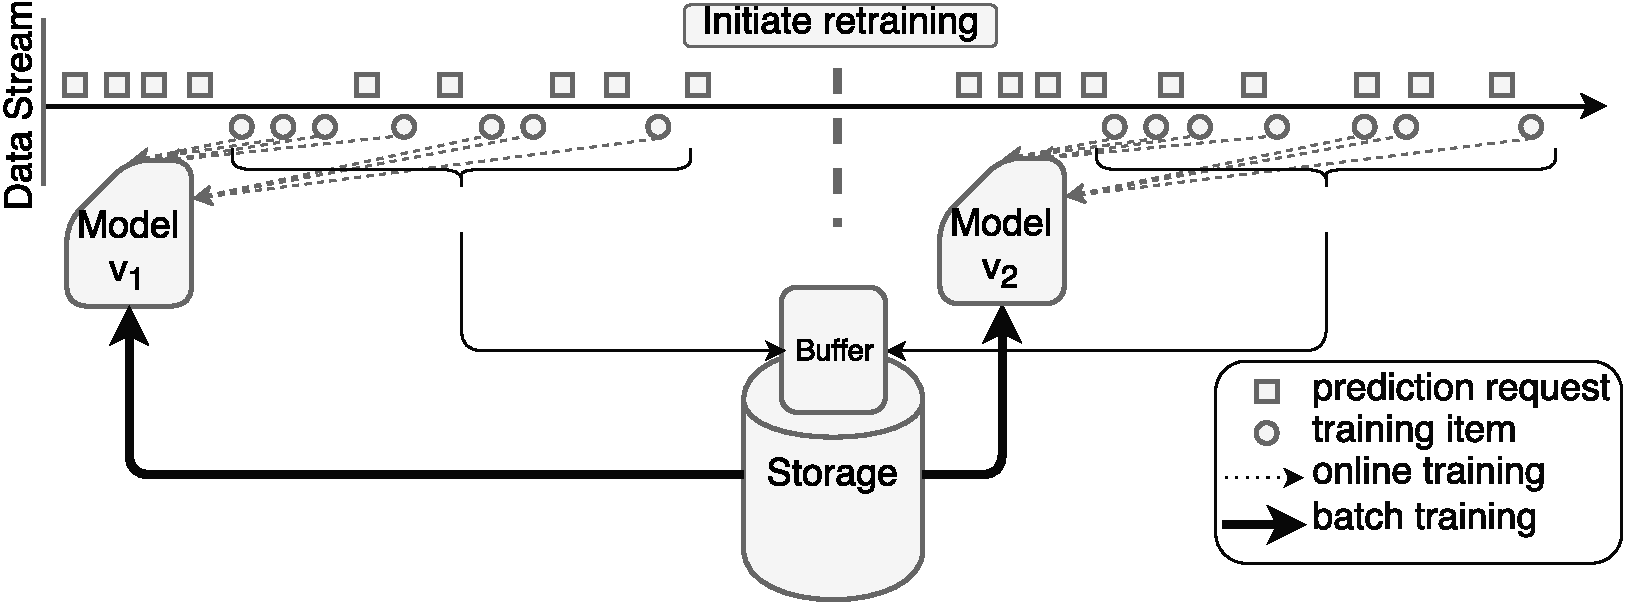
\includegraphics[width=1\columnwidth]{../images/velox-final.pdf}
%\caption{Current Model Deployment Method}
%\label{fig:velox-work-flow}
%\end{figure}


\section{Related Work} \label{related-work}
Traditional machine learning systems focus solely on training models and leave the task of deploying and maintaining these models to the users.
It has only been recently that some systems, for example Velox \cite{crankshaw2014missing}, TensorFlow Serving \cite{abadi2016tensorflow}, and LongView \cite{akdere2011case} have proposed architectures that also consider model deployment and query answering.
LongView integrates predictive machine learning models into relational databases. 
It answers predictive queries and maintains and manages the models.
LongView uses techniques such as query optimization and materialized view selection to increase the performance of the system.
However, it only works with batch data and does not provide support for real-time queries. 
As a result it does not support incremental learning.
In contrast, our system is designed to work in a dynamic environment where it answers prediction queries in real-time and incrementally updates the model when required.
TensorFlow Serving provides mechanisms for real-time queries, deployment and version control of machine learning models.
It has out-of-the-box support for models created using TensorFlow and provides several interfaces for users to deploy their custom models.
However, it does not provide incremental updates to the model.
Contrary to our system, models have to be retrained outside of the system and have to be redeployed to TensorFlow Serving once the training is complete.
Our system supports incremental and batch updates to the model and automatically applies these updates to the model currently being served.

Velox is an implementation of the common machine learning serving practice \cite{crankshaw2014missing}, explained in Section \ref{introduction}.
Velox supports incremental learning and can answer prediction queries in real-time.
It also eliminates the need for users to manually retrain the model offline and redeploy it again.
Velox monitors the error rate of the model using a validation set.
Once the error rate exceeds a predefined threshold, Velox initiates a complete retraining of the model using Spark. 
This deployment method, however, has three drawbacks; retraining discards updates that have been applied to the model so far, the process of retraining on full data set is resource intensive and time consuming, and new datasets introduced to the system only influence the model after the next retraining.
Our approach differs, as it exploits the underlying properties of SGD to fully integrate the training process into the system's lifeline.
This eliminates the need for completely retraining the model and replaces it with consecutive SGD-iterations.
Moreover, our system can train the model on new batch datasets as soon as they become available.

Clipper \cite{crankshaw2016clipper} is another machine learning deployment system that focuses on producing higher quality predictions by maintaining an ensemble of models.
It constantly examines the confidence of each model.
For each prediction request, it uses the model with the highest confidence.
However, it does not incrementally train the models in production, which over time leads to models becoming outdated.
Our deployment method on the other hand, focuses on maintenance and continuous updates of the models.

Weka \cite{hall2009weka}, Apache Mahout \cite{Owen:2011:MA:2132656}, and Madlib \cite{hellerstein2012madlib} are systems that provide the necessary toolkits to train machine learning models. 
All of these systems provide a range training algorithms for machine learning methods. 
However, they do not provide any management, before or after the models have been deployed. 
Our proposed system focuses on models trainable using stochastic gradient descent and as a result is able to provide model management both during training and deployment time.

MLBase \cite{kraska2013mlbase} and TuPaq \cite{sparks2015tupaq} are model management systems.
They provide a range of training algorithms to create machine learning models and mechanism for model search as well as model management.
They focus on training high quality models by performing automatic feature engineering and hyper-parameter search.
However, they only work with batch datasets.
Once models are trained, they have to be deployed and used for serving manually by the users.
Our system, on the contrary, is designed for deployment and maintenance of already trained models.

\section{Stochastic Gradient Descent} \label{sgd}
\todo[inline]{Schelter: rewrite!!}
Machine learning minimizes an objective function (often referred to as the loss function).
Usually, this requires us to calculate the gradient of the function at different data points and update the function parameters based on the gradient values.
A common optimization method is gradient descent, an iterative process where each iteration uses the entire training data set to calculate the gradient value.
One drawback of gradient descent is that in presence of large datasets it performs very slow.
Stochastic gradient descent \cite{bottou2010large} is an approximation of the gradient descent method. 
Similar to gradient descent, it is an iterative process.
However, in each iteration it calculates the gradient at a single element (or a small sample) and updates the parameters of the model accordingly. 
Although it converges after a higher number of iterations, the overall convergence time is lower (sometimes by orders of magnitude) than gradient descent \cite{bottou2010large}. 
Each iteration of SGD executes in a short amount of time because it only works with a sample of the data.
We are leveraging this property of SGD and design our deployment system so that it performs one iteration of SGD at a time without interrupting the query answering component.
In Section \ref{evaluation}, we show that the overhead from executing a single iteration of SGD is very small and does not affect the query answering component.

\subsection{Distributed SGD}
To efficiently train machine learning models on large datasets, scalable techniques have to be employed.
SGD inherently works well with large amounts of data because it does not need to scan every data point during every iteration.
However, for very large datasets, SGD has to perform many iterations in order to converge.
To decrease the running time, large datasets can be distributed among multiple nodes, where each node will compute the gradients on a subset of the data in parallel.
One drawback of this approach is that a synchronization step is required before applying the updates to the model, which slows down the optimization process.
To alleviate this, several asynchronous SGD methods are proposed \cite{recht2011hogwild, dean2012large}. 
\hl{Experiments using these methods show that the quality of the produced model in some cases is similar to the synchronized SGD approach.}

\subsection{Machine Learning Models based on SGD}\label{subsec:ml-models-sgd}
SGD is a common optimization methods that has been used in classification \cite{zhang2004solving}, clustering \cite{bottou1995convergence}, neural networks \cite{dean2012large}, and matrix factorization \cite{funk2006netflix}.
Some examples of machine learning models that use SGD are: 

\textbf{Linear Classifiers} are arguably the most common type of machine learning models built using the SGD optimization method. 
In the CTR prediction example of Section \ref{introduction}, we use logistic regression to train the model for predicting the click through rate \cite{macmahan2013}. 
Logistic regression models typically output a probability instead of a class label that indicates how likely an item belongs to a specific class \cite{hosmer2013applied}.
In our example, logistic regression predicts the click probabilities for all the available advertisements and the ones with the highest probabilities are displayed.
Support vector machines (SVM) represent another common class of classification models \cite{steinwart2008support}.

\textbf{Matrix Factorization} is a common method used in recommender systems \cite{koren2009matrix}. 
Matrix factorization is used to derive the latent factors (e.g., for users and items) for recommender systems.
It relies on the fact that each user and item can be described in a few dimensions (10 to 40 usually) based on the available ratings.
These latent factors automatically capture the similarity of users and items based on the ratings provided by the users.
Hence, any unknown rating can be predicted by computing the dot product of the user vector with the item vector.

\textbf{Neural Networks} or deep learning -- inspired by biological neural networks in the brain -- are used to learn and approximate complex functions. 
They have been used for more than half a century to model functions and have been successfully applied to training machine learning models.
However, due to the slow training process and the lack of large amount of training data, they have not been used extensively in the machine learning community in the past.
In the last decade, there was a drastic change due to several seminal publications.
Hinton et al. proposed methods for speeding up the training of neural networks \cite{hinton2006fast}.
The ImageNet competition \cite{ILSVRC15} in 2012 was won by a neural network proposed by Krizhevsky et al. where they significantly reduced the error rate \cite{krizhevsky2012imagenet}. 
The success of the Google's Deepmind team in achieving Neural Networks that were capable of defeating humans in the game of Go \cite{silver2016mastering} and mastering Atari games \cite{mnih2013playing} was also instrumental in popularizing neural networks in the machine learning community.

SGD is the ideal optimization algorithm for training neural networks since it works very well with large datasets (which are required for training neural networks).
In fact, almost all recent work on neural networks uses SGD for training them.
\todo[inline]{Schelter: too much blabla, not ....}

\begin{figure}[t]
\centering
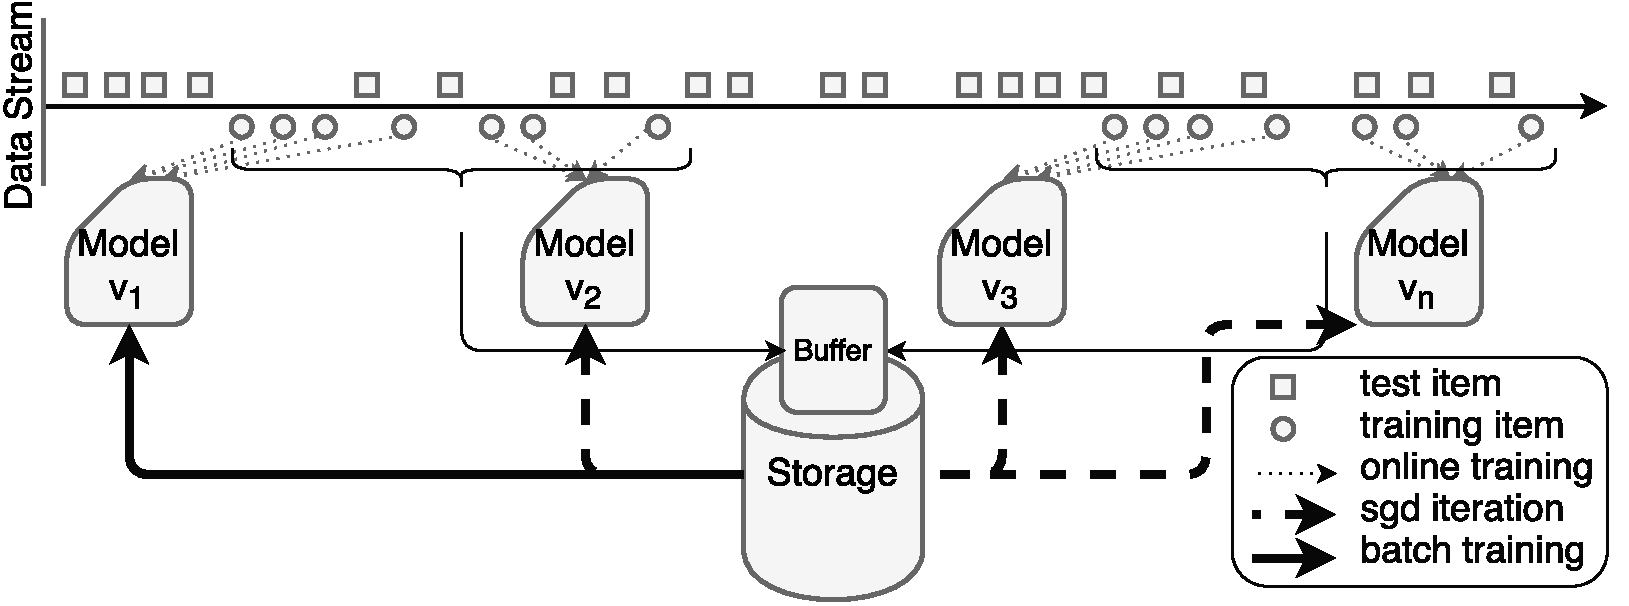
\includegraphics[width=\columnwidth]{../images/continuous-final.pdf}
\caption{Continuous Training and Serving}
\label{fig:cont-training-serving}
\end{figure}

\section{Continuous Training and Serving} \label{continious-training-serving}
Our proposed deployment and maintenance system uses SGD as its underlying learning algorithm.
As a result, it can update the model incrementally (one training item at a time) or use mini-batches of data.
\todo[inline]{schelter: awful?}
The core design principles of our deployment system are threefold.
First, we incrementally update the model so that it can adapt to changes in the distribution of the incoming data.
Second, we eliminate retraining and replace it with a series of consecutive iterations of SGD.
And finally, we immediately use new batch datasets that are available to the system.
Figure \ref{fig:cont-training-serving} shows how our deployment method works.
First, using the existing data residing on disk, we train an initial model and deploy it into the system.
The system receives prediction queries and training observations in a streaming fashion.
The deployed model answers incoming prediction queries as soon as they are received.
Once the system receives a training observation it updates the model incrementally.
The system also keeps track of incoming training observations and adds them to an intermediate buffer.
A scheduler component, triggers new iterations of SGD based on the rate of incoming training observations. 
The scheduler can also decide to run an iteration when the system is not under heavy load.
Each new iteration uses a random sample of the data in storage and the data in the buffer. 
Moreover, our system stores new batch datasets in the buffer (or the persistent storage unit) as soon as they become available.
Any further scheduled iteration of SGD incorporates the new data without requiring the model to be retrained from scratch.

\todo[inline]{R3: Section 5 has many unclear and informal descriptions, without formal methodology.}
\section{System Architecture} \label{sec:system-architecutre}
\begin{figure}[t]
\centering
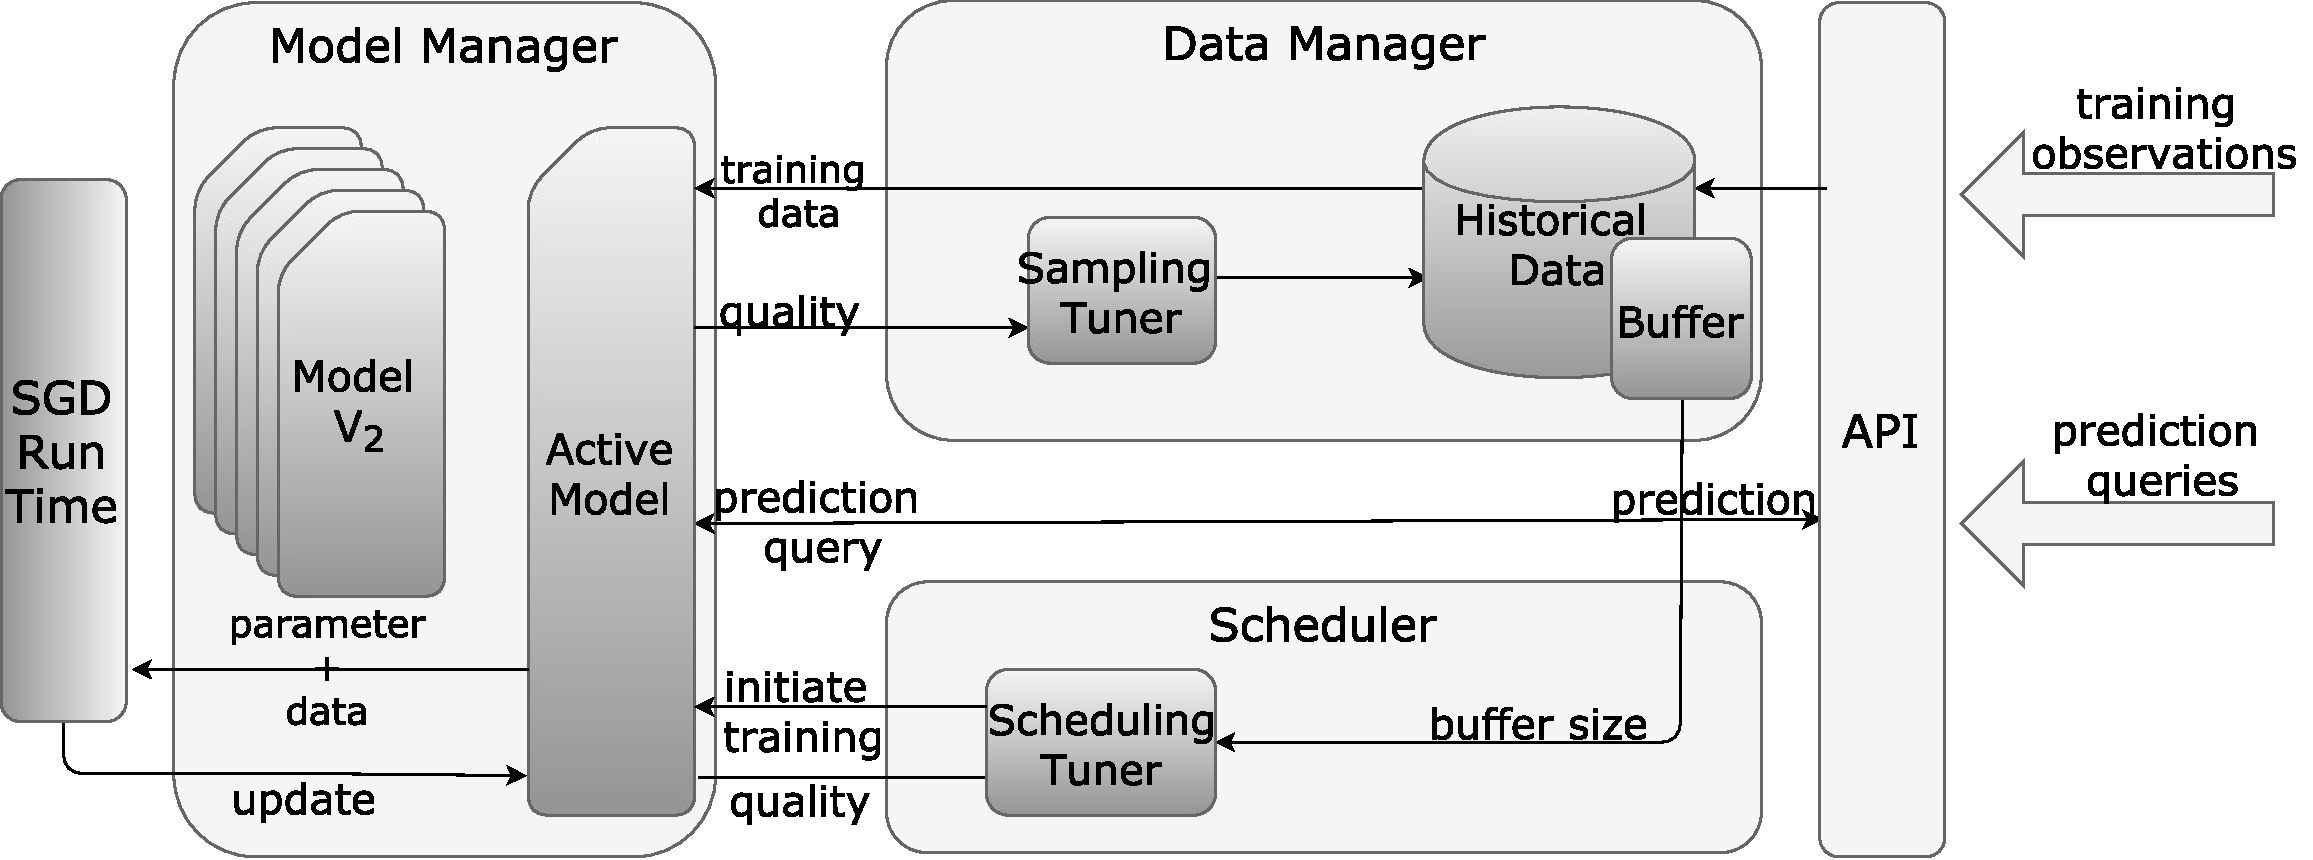
\includegraphics[width=\columnwidth]{../images/system-architecture-final.pdf}
\caption{System Architecture}
\label{fig:system-architecture}
\end{figure}

The proposed system comprises three main components; model manager, data manager and scheduler, and an independent SGD run-time. 
Figure \ref{fig:system-architecture} gives an overview of the architecture of our system and the interactions among its components.
The data manager first stores the incoming training observations in a buffer and then passes them on to the model manager.
The model manager incrementally updates the model using the training observations.
The model manager is also responsible for receiving prediction requests.
Once it receives a request, it uses the latest version of the model to make a prediction and returns the result to the user.
Both the scheduler and the data manager components are constantly communicating with each other and with the model manager, to obtain the latest statistics, such as the model quality and buffer size.
This in turn helps us to tune the scheduling and sampling rate for future iterations of SGD. 
Next, we explain each component of the system in more detail.

\subsection{Scheduler}\label{scheduler}
The scheduler component is responsible for scheduling new iterations of SGD.
Intuitively, the best time to execute an iteration is when the system is not under heavy load.
A new iteration of SGD is also executed when the system receives more training data than can be handled by the intermediate buffer.
If the model is not updated with the new training items frequently, the quality decreases.
This decrease in the quality is more rapid if the distribution of the data is changing.
In our prototype, the scheduling rate is controlled by a user defined parameter, \textit{max\_buffer\_size}.
When the intermediate buffer's size reaches \textit{max\_buffer\_size}, the scheduler executes a new iteration of SGD.
It is important to note that the scheduling rate affects the quality of the model.
In Section \ref{evaluation}, we investigate the effect of scheduling rate on model quality.
If no new training data is available, the model parameters will eventually converge and any further training iterations will not have any effect on the model quality.
\todo[inline]{R3: How is the convergence detected?}
Therefore, the scheduler component has to communicate with the model manager in order to detect whether the model parameters have converged and stop further iterations until more training data becomes available.

\subsection{Data Manager} \label{data-manager}
In order to execute an iteration of SGD, we need to combine the training data that arrives at the system in real-time with the data stored on disk.
The data manager is responsible for storing the incoming training observations in an intermediate buffer.
Upon a new training iteration, the data manager accesses the historical data stored on disk and provides a sample.

Different sampling strategies can be used to provide the sample.
In our current prototype, the data manager uses a simple unified random sampling method to generate this sample.
More advanced methods, such as Reservoir \cite{vitter1985random} or weighted random sampling can also be used to generate the sample.
Reservoir sampling is typically used to generate samples from large datasets that do not fit in memory, whereas weighted random sampling is used when data elements have different weights.
In an online machine learning scenario, recent items are more important for training the model and are assigned a bigger weight than older items.
Therefore, weighted random sampling can generate samples that can contribute to the training of a better model.

The data from the sample and the data in the buffer are merged to create the dataset for next training iteration.
The data manager provides access to this dataset for the model manager in order to further train the model.
The data manager also communicates with the scheduler in order to inform it when the intermediate buffer is becoming full and a new training iteration is required. 

The created data set consists of the data inside the buffer and a sample of the historical data as described earlier.
The sampling rate is a system parameter that has to be configured.
It can be pre-configured to a constant value based on the application.
However, using the feedback from the system's model manager (Section \ref{model-manager}), the sampling rate can be adjusted.
For example, when the data distribution is changing, a smaller sampling rate places more emphasis on the data that arrived recently. 
This is similar to the problem of concept drift where the distribution of the incoming data changes overtime.
This renders historical data less important and as a result a smaller sample of the historical data (or none at all) will give more importance to the data in the buffer and help the model to adopt faster to the concept drift.
However, if there is no concept drift in the data, a larger sampling rate will increase the quality of the model after a training iteration.
Another effect that the sampling rate has on the system is the training iteration running time.
A larger sampling rate increases the running time of each training iteration as more data has to be processed.
In Section \ref{evaluation}, we investigate the effects of different sampling rates on both the quality and performance of the system.

Moreover,  new data sets can be registered in data manager.
In our current prototype, new data sets first have to be stored on disk, and data manager can be informed of the data path.
Newly available data sets are used in the subsequent SGD iterations.

\todo[inline]{R2: The difference of incremental update and SGD update needs clarification. In the experiment, they are used in different approaches (baseline+ is using incremental update and Continuous is using SGD). But, the second sentence of the last paragraph of sec 5.3 says both updates are applied in Continuous. BD: I have used incremental to refer to online learning. Whereas in some literature incremental may also refer to mini batch updates. I think the reviewers comment is already addressed in section \ref{subsec:setup}}
\subsection{Model Manager} \label{model-manager} 
An important part of the system is the model manager component.
It is responsible for storing the model, answering prediction queries, and performing incremental and batch updates to the model.
Listing \ref{model-manager-api} shows the API of the model manager.
The API is used to interact with other components as well as end-users of the system.
The scheduler component uses \textit{update} and \textit{update\_iteration} to instruct the model manager to perform incremental or batch updates (one iteration of SGD) to the model.
Upon a new prediction query, the \textit{predict} method is called to provide the end-user with the label of the given input.

\noindent\begin{minipage}[t]{\linewidth}
\begin{lstlisting}[language=java, basicstyle=\small\ttfamily, frame=tb ,columns=fullflexible,
showstringspaces=false,label=model-manager-api,caption=Model Manager API, numberstyle=\tiny]
def update(x,y)

def update_iteration(X,Y)

def predict(x): Label

def error_rate(X_test, Y_test): Double

\end{lstlisting}
\end{minipage}


The \textit{error\_rate} method returns the error rate of the model using the provided test dataset.
As described earlier, constant monitoring of the quality is required in order to adjust the scheduling and sampling rate.
When the error rate is stagnating, the model has converged using the existing data.
Therefore the model manager informs scheduler not to schedule any new iterations until new training observations have arrived at the system.
\todo[inline]{R3: How is this done exactly?}
Similarly as explained in Section \ref{data-manager}, an increase in the error rate may indicate a change in distribution of the data.
As a result, reducing the sampling rate will place more emphasis on recent data (in the intermediate buffer) and help adapt the model to the changes in the distribution.

The model manager also keeps track of the changes that are made to the model.
The model is updated both through incremental learning and SGD-iteration.
The model manager creates snapshots of the model in two different scenarios; after a series of incremental updates are made and after each training iteration.
\todo[inline]{R3: What is the algorithm here?}
This versioning of the models is essential.
When there is a rapid change in the distribution of the incoming data (a sudden concept drift) or when there are anomalies in the data, it is sometimes necessary to revert back to a version before the change in distribution occurred.
In case of concept drift, new training iterations should be scheduled that only use the data in the buffer.
Moreover, in case of anomalies in the data, they have to be identified and discarded before any further model updates could happen.

\subsection{SGD Run-Time} 
All components of our model serving system described so far are not limited to any specific run-time.
We have decoupled the components from the actual run time of the system.
Any system capable of performing incremental and batch SGD updates efficiently are suitable options for our system.
Apache Flink \cite{carbone2015apache} and Apache Spark \cite{zaharia2010spark} are distributed data processing platforms that work with data in memory and have support for iterative algorithms, which makes both of them ideal options for our SGD run-time.
In our current prototype, we are using Apache Spark \cite{zaharia2010spark} as our SGD run-time.

The model manager is the component responsible for communicating with the SGD run-time.
In the current version of our prototype, the model manager requests Spark to perform both incremental and batch updates to the model.
Both types of updates are supported by the built in machine learning library of Spark.
The choice of run-time for SGD slightly influences the data manager as well.
In our prototype, historical data is stored on the Hadoop Distributed File System (HDFS) \cite{shvachko2010hadoop}.

\todo[inline]{R3: The paper has a point that not only the resource consumption is reduced by incremental update, but also the prediction accuracy can be improved due to adapting the model to newly seen data. The system uses a sampling component to use a subset of historical data in each SGD update. However, a non-incremental retraining can also achieve the same adaptation by weighing towards the newly seen data (e.g., learning with concept drifting). Therefore, the ideas of incremental update and adaptation to concept drift should not be confused. The evaluation in this paper does not clearly decouple them. BD: Interesting insight. We have to address this.}
\section{Evaluation} \label{evaluation} 
In this section we evaluate the performance of our system using various datasets. 
We report both the quality (error rate) and performance of our proposed method. 

\subsection{Setup}\label{subsec:setup}
We evaluate our deployment method in distributed environment consists of 11 nodes (1 master, 10 slaves).
Each node is running on an Intel Xeon 2.40 GHz 16 core processor and has 28 GB of dedicated memory for running our prototype.

We implement a prototype of our deployment method on top of Apache Spark \cite{zaharia2010spark}.
It uses the SGD implementation available in the machine learning library of Apache Spark.
To demonstrate the deployment platform designed two machine learning pipelines.

\textit{Criteo pipeline.} The Criteo pipeline consists of 5 operations: missing value imputer, column indexer, one hot encoder, vectorizer, standard scaler, and logistic regression model trainer. 
The Terabyte Criteo click log dataset is used for benchmarking algorithms for clickthrough rate (CTR) prediction \cite{criteo-log}.
It contains \hl{24} days of user click logs. 
The dataset  contains 13 numerical and 26 categorical features. 
After applying the indexer and one hot encoding number of features increased to \hl{1,000,000}.

\textit{XXX pipeline.} 

For all of the classification datasets, we report the prequential error when receiving a new training instances \cite{gama2009issues} .

\textit{Deployment scenario.} 
Pipelines are trained on an initial part of the data and then continuously trained using the remaining of the data.
We define 3 different deployment scenarios.
\begin{itemize}
\item A: Periodical retraining with no statistics collection
\item B: Periodical retraining with statistics collection
\item C: Proactive training with statistics collection
\end{itemize}

For Criteo pipeline, the pipeline is retrained on a daily basis.

\subsection{Tuning parameters} \label{tuning}
In Section \ref{continious-training-serving}, we discussed how system parameters such as sampling and scheduling rate affect the performance and quality of the system.
In this section, we analyze the effects of different sampling and scheduling rates on the system.

\textbf{Scheduling rate:} 
\todo[inline]{redo this part using the criteo dataset}
This parameter specifies how often a new iteration of SGD should be scheduled. 
In our prototype, the scheduling rate is governed by a parameter called buffer size, which dictates how many new items should be stored in the buffer before a new iteration of SGD is executed. 
Executing one iteration of SGD, even using the entire data, is not a resource heavy process, and can be executed simultaneously with the serving component of the system. 

\begin{figure}[h]
\begin{subfigure}{\columnwidth}
\centering
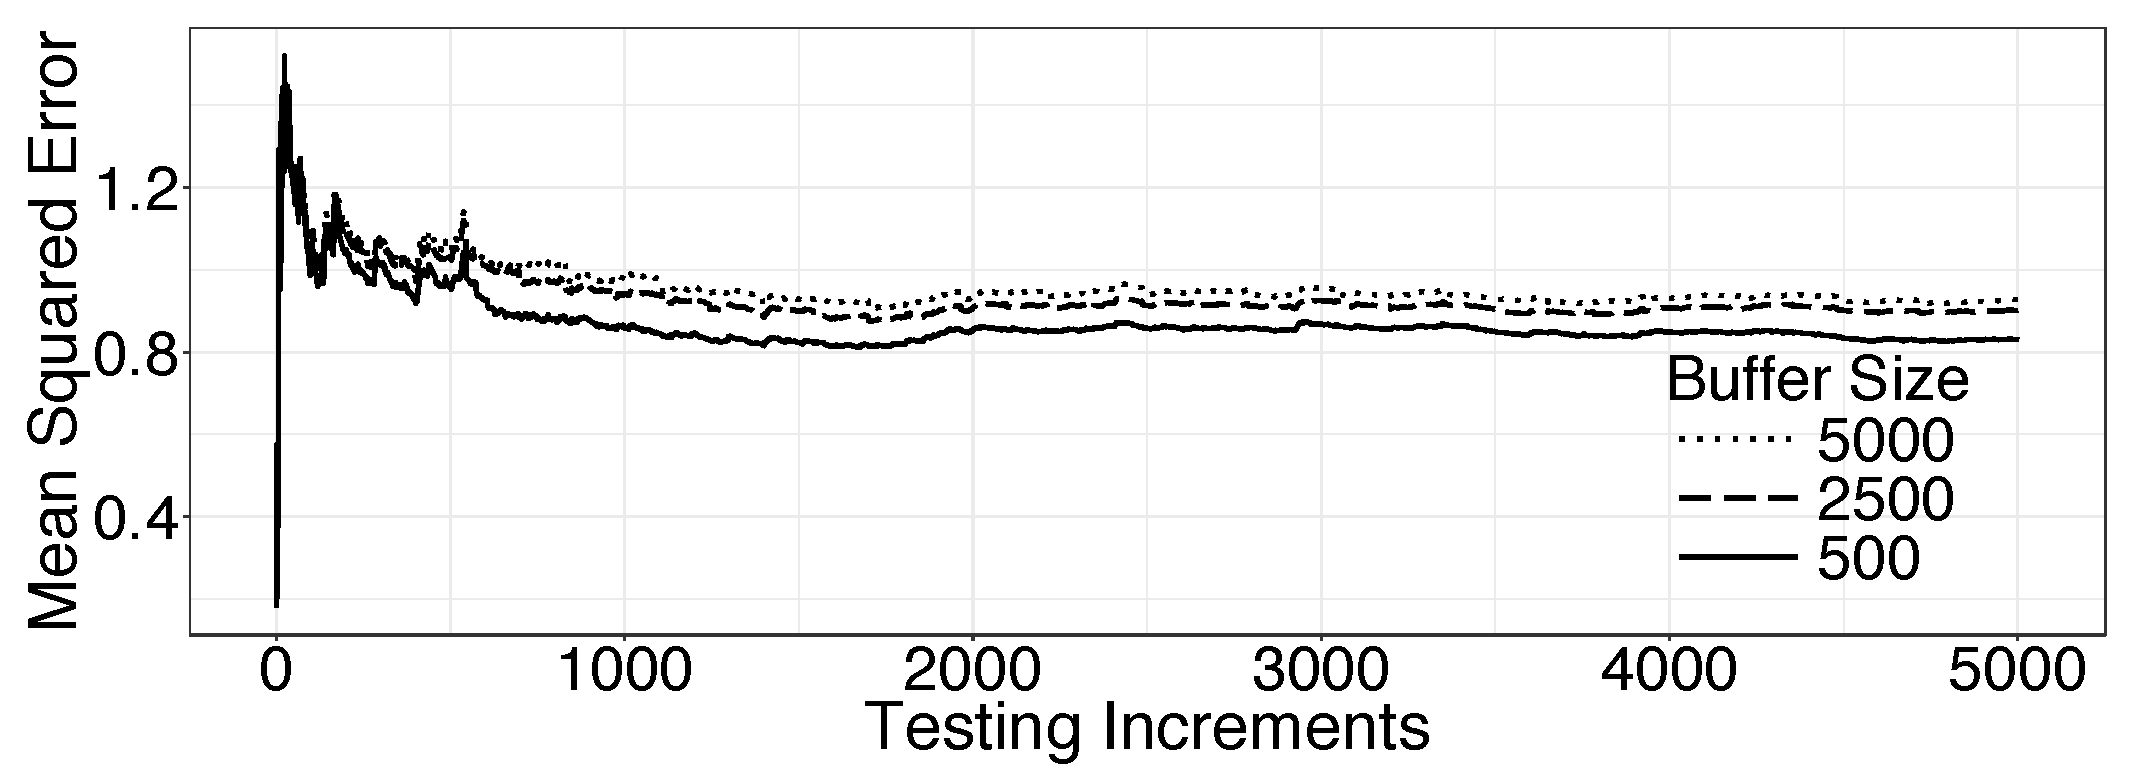
\includegraphics[width=\columnwidth]{../images/experiment-results/movie-lens-buffer-quality-improved.eps}
\caption{Buffer size}
\label{fig:movie-lens-100k-buffer-size-mse}
\end{subfigure}
\begin{subfigure}{\columnwidth}
\centering
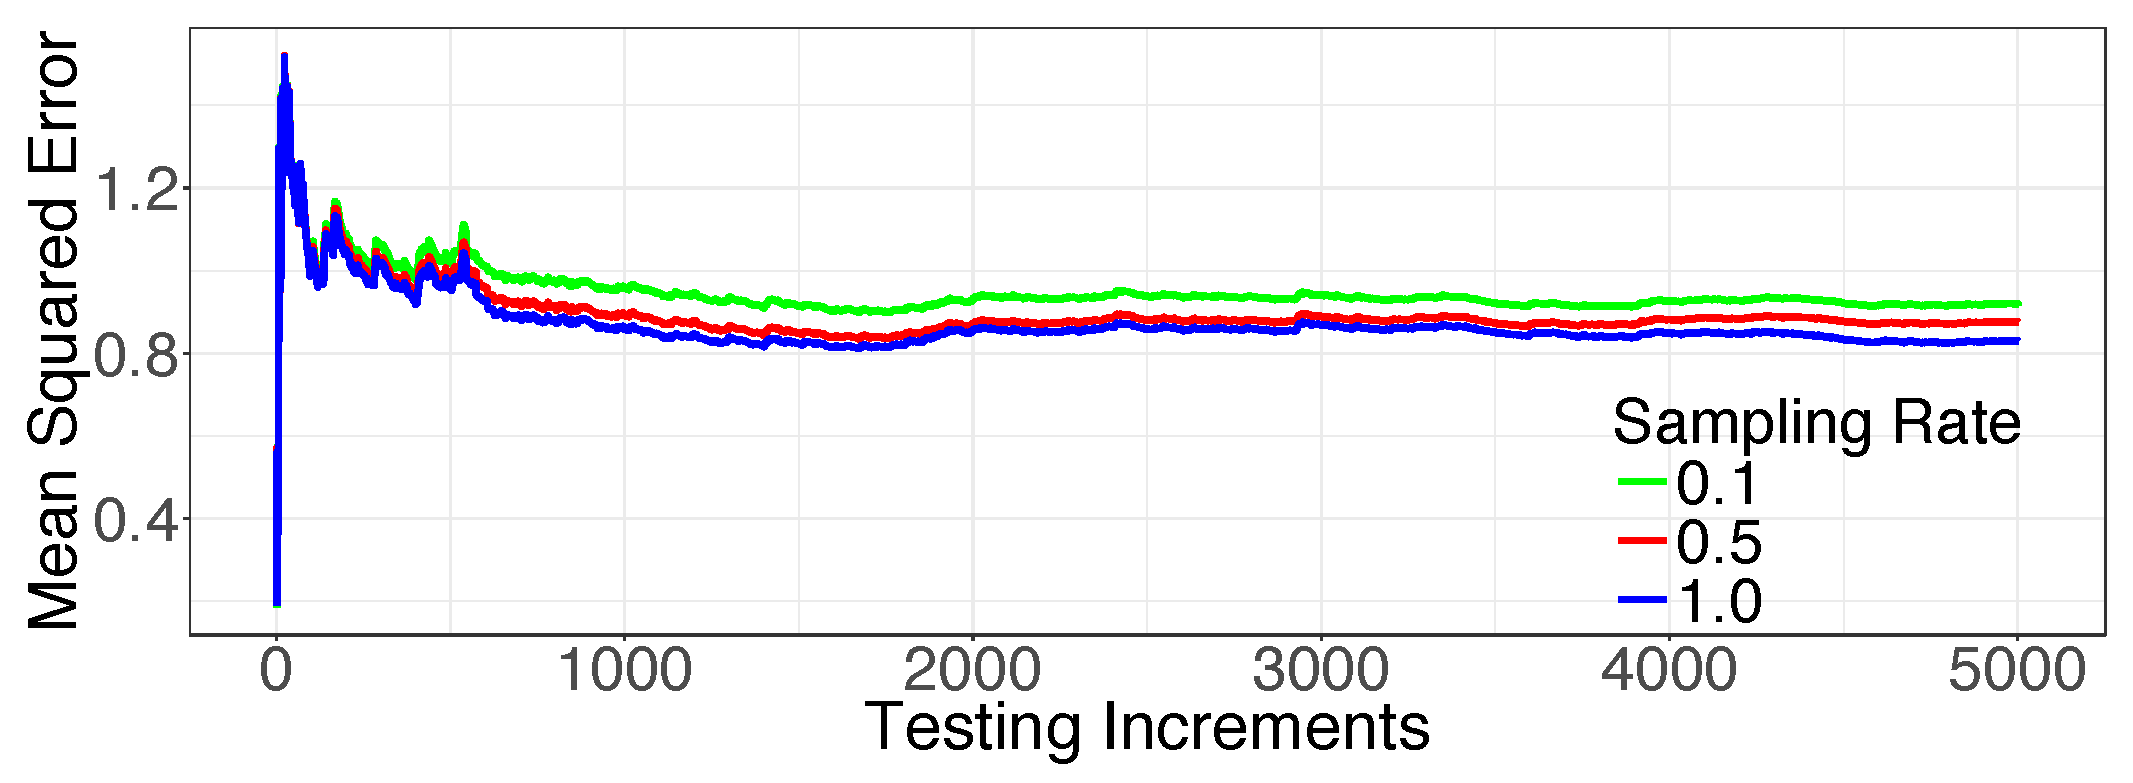
\includegraphics[width=\columnwidth]{../images/experiment-results/movie-lens-sampling-quality-improved.eps}
\caption{Sampling rate}
\label{fig:movie-lens-100k-sample-rate}
\end{subfigure}
\vspace{2mm}
\caption{Effect of Sampling and Scheduling Rate on Quality (Movie Lens 100K)}
\end{figure}

Figure \ref{fig:movie-lens-100k-buffer-size-mse} shows the mean squared error for different buffer sizes for Movie Lens 100k. 
A smaller buffer size forces the scheduler to initiate training iterations more frequently.
As a result, the system updates the underlying model more often.
However, the error rate is not decreasing linearly with the buffer size.
Further analysis shows that the more frequent the model updates are, the faster the model converges and any further training has little to no effect on the overall quality.
This is extremely important, specially when considering the effect of the buffer size on the running time.
Figure \ref{fig:movie-lens-100k-buffer-size-time} shows the running time on Movie Lens 100k using different buffer sizes. 
Increasing the buffer size from 500 to 5000 decreases the running time by a factor of 5 while the MSE is only decreased slightly.
Therefore, depending on the application, we can set the buffer size to bigger values in order to increase the performance of the system without affecting the quality of the final model substantially.

\begin{figure}[H]
\begin{subfigure}{0.5\columnwidth}
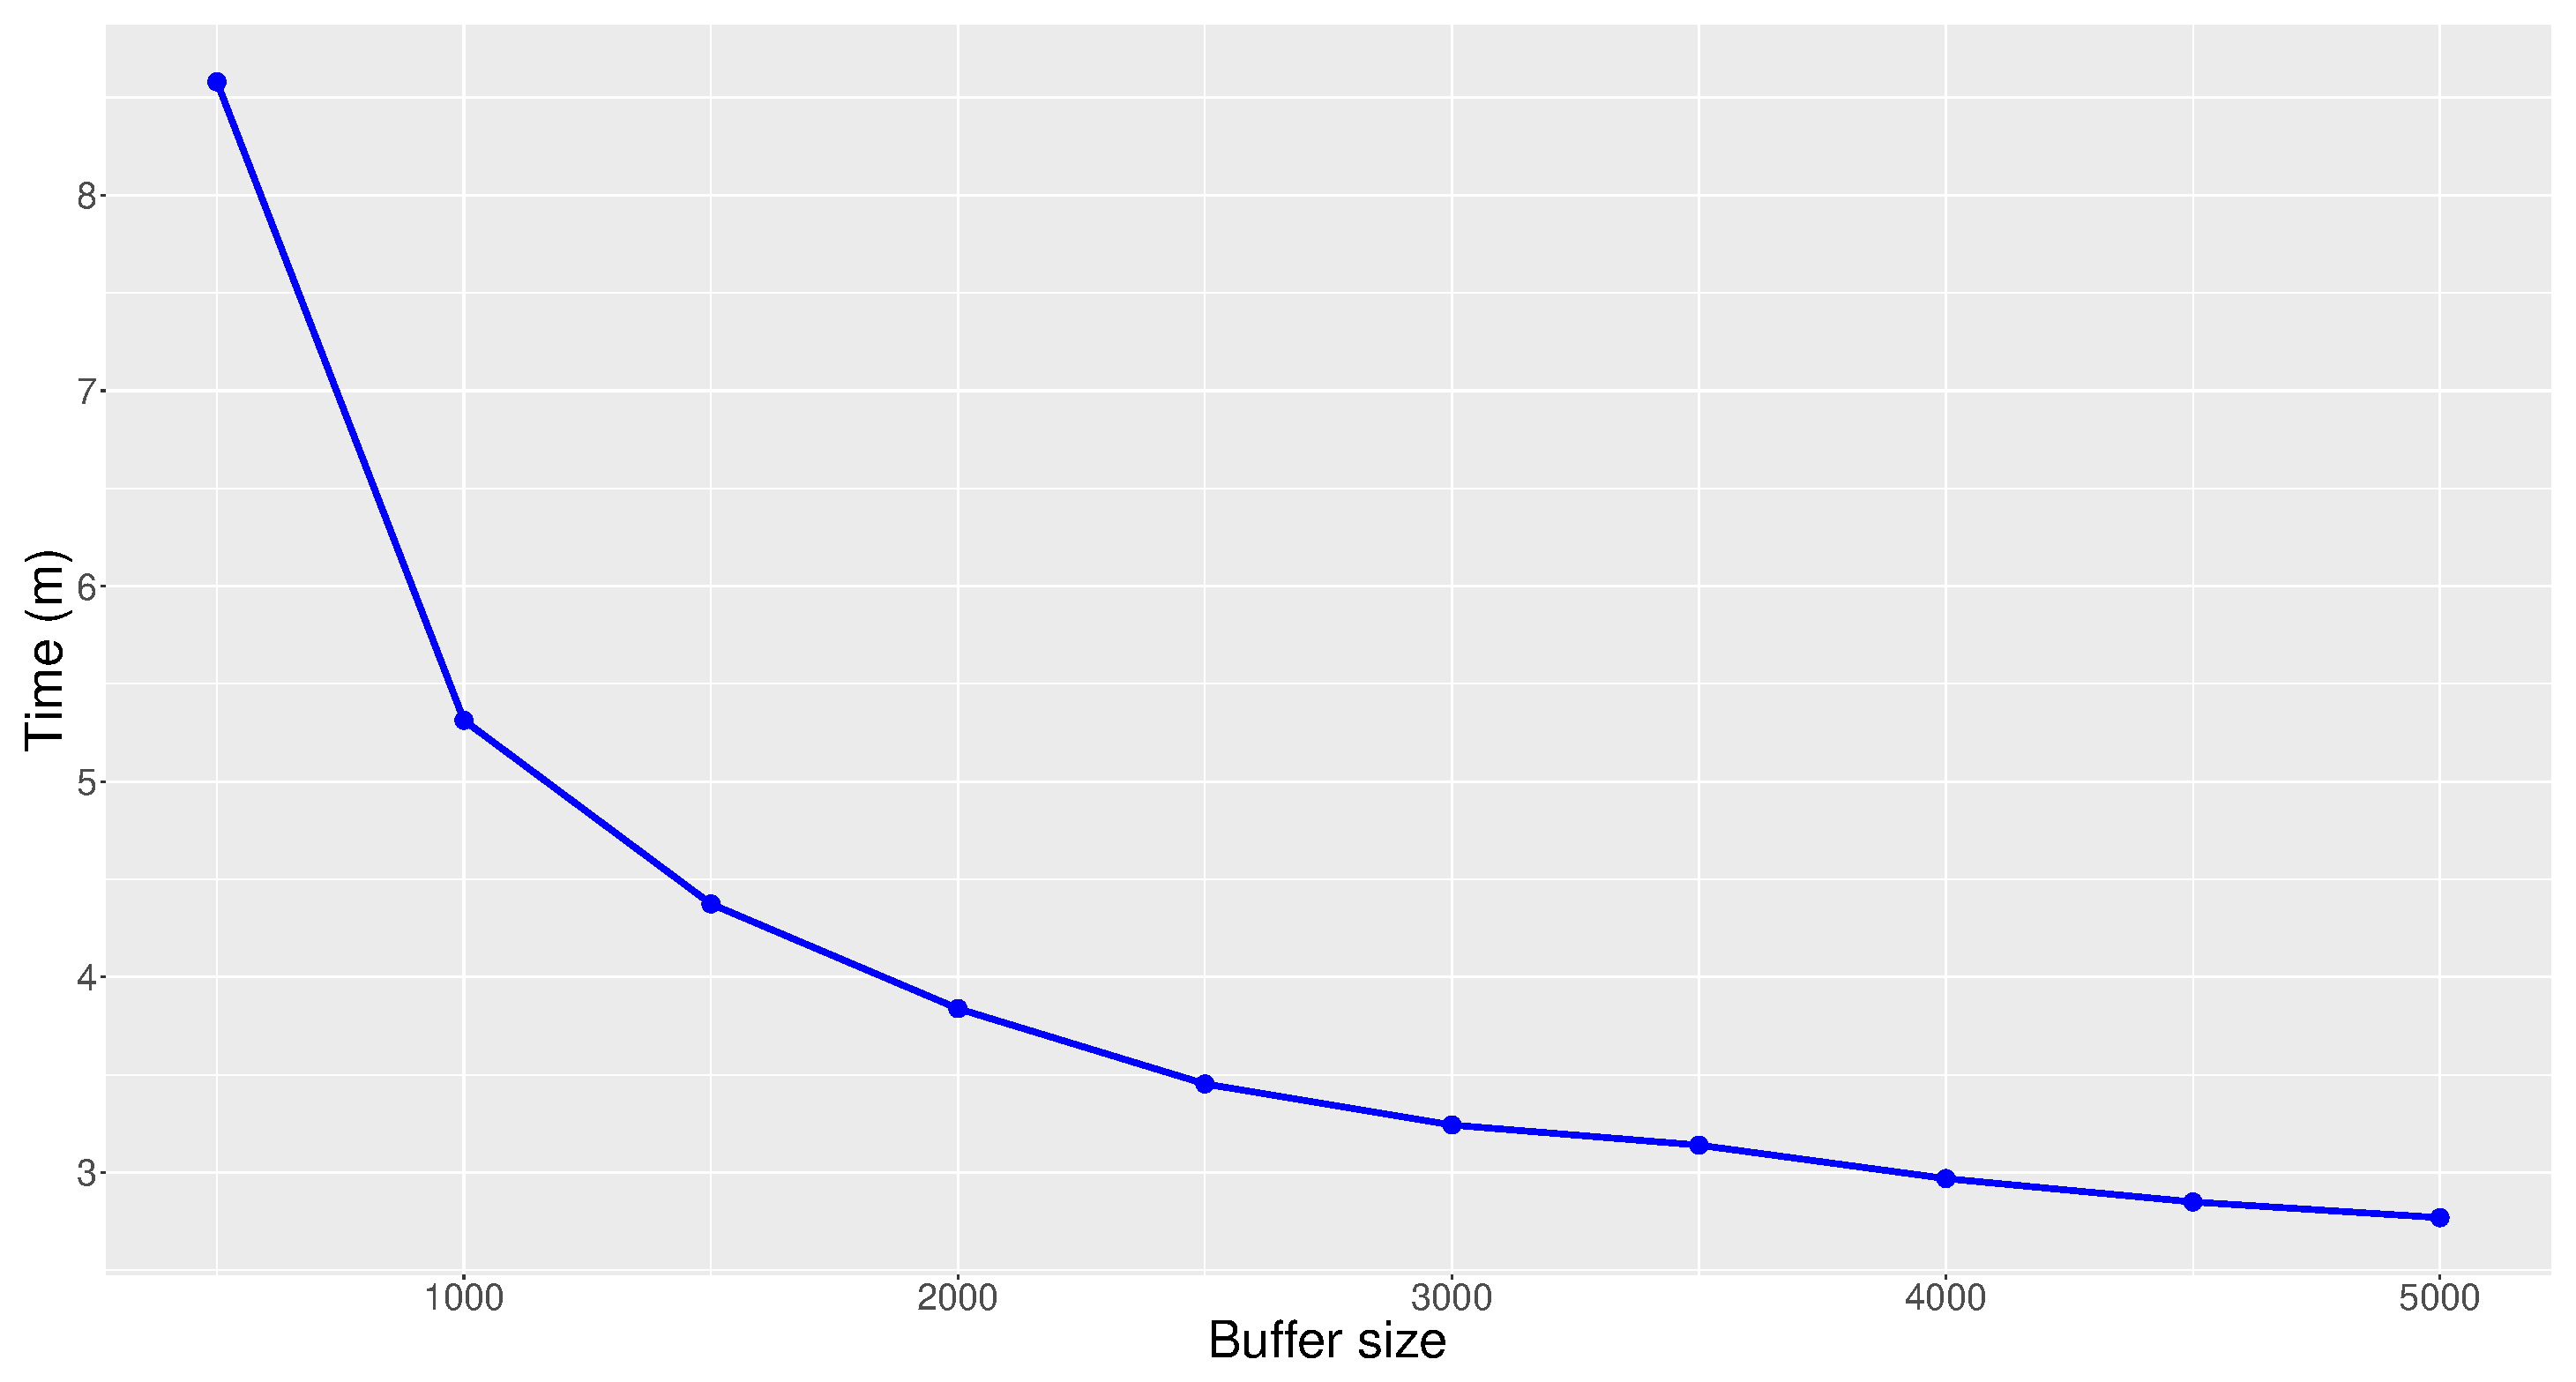
\includegraphics[width=\columnwidth]{../images/experiment-results/movie-lens-100k-buffer-time-improved.eps}
\caption{}
\label{fig:movie-lens-100k-buffer-size-time}
\end{subfigure}%
\begin{subfigure}{0.5\columnwidth}
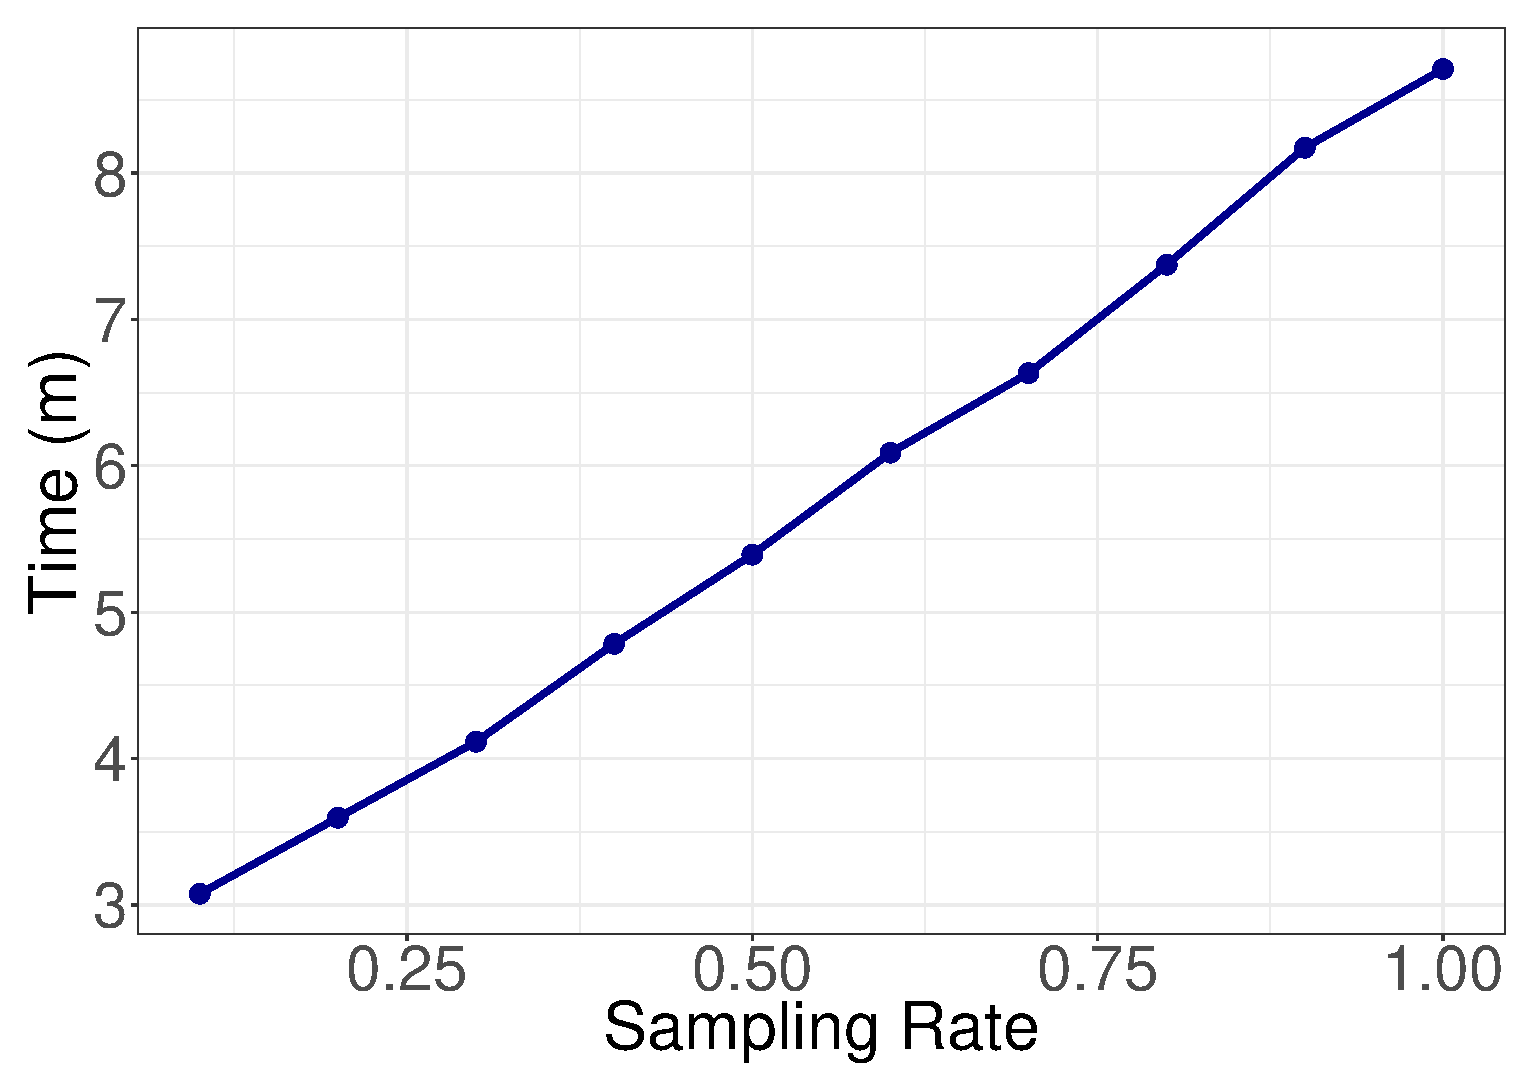
\includegraphics[width=\columnwidth]{../images/experiment-results/movie-lens-100k-sampling-time-improved.eps}
\caption{}
\label{fig:movie-lens-100k-sample-rate-time}
\end{subfigure}
\vspace{2mm}
\caption{Effect of Sampling and Scheduling Rate on Running time (Movie Lens 100K)}
\end{figure}

\todo[inline]{R1: Dynamic Scheduling is an interesting idea -- but you're not offering any scheduling algorithm here? Just the idea that you can schedule training when there's free CPU cycles? BD: Scheduling and Sampling rate have to be studied in more detail. All reviewers had concerns about these}
\todo[inline]{R3: What is exactly the scheduling?}
\textit{Dynamic scheduling:} In production environments, the load on the system typically varies throughout the lifetime of the application.
Therefore, a dynamic scheduling maximizes the performance of the system, by performing more frequent updates while there are more resources available for training. 
\todo[inline]{R1: "Moreover, since training and serving ... only update the weights when the training iteration is over". Why? Why not apply the updates to the model in-place? This allows you to serve every request with the absolute freshest model. At least for the single-machine case. BD: the updated model is the result of the training iterations, therefore, we have to wait until the iteration is over. The sentence seems clear to me. I should it run it by TR}
Moreover, since training and serving can be done in parallel, we can perform training in a background process and only update the weights when the training iteration is over. 

\textbf{Sampling rate:} 
\todo[inline]{redo this part, compare weighted time-based sampling vs random sampling different sizes}
In each iteration of SGD the data inside the buffer and a sample of the historical data is combined to update the model.
In this section, we investigate the effect of the sampling rate on the model quality and the running time of the system.
Figure \ref{fig:movie-lens-100k-sample-rate} shows that a larger sampling rate increases the quality of the model.
However, similar to the scheduling rate, the decrease in error rate is negligible considering the effect it has on running time. 
This is caused by the same phenomena, where the model after training on bigger sample rates start to converge faster.
As a result, bigger sample sizes do not have a considerable effect on the quality.
 
Figure \ref{fig:movie-lens-100k-sample-rate-time} shows the effect of increasing the sampling rate on the running time.
Increasing the sampling rate from 0.1 to 1.0, increases the running time by a factor of 5.
\todo[inline]{R3: . The sampling parameter deserves a more systematic treatment since it deeply affects the performance. In fact, Baseline+ and Velox represent two extreme settings of it: 0\% and 100\%. Instead, the paper simply suggests "setting the sampling rate to smaller values will increase the performance substantially, while only slightly affecting the quality of the model." It is not a sound conclusion if we agree Baseline+ is equivalent to 0\% sampling rate.}
Therefore, similar to the scheduling rate, setting the sampling rate to smaller values will increase the performance substantially, while only slightly affecting the quality of the model.

\textbf{Tuning parameters based on error rate:} The underlying machine learning model and the dataset have big effects on the selection of sampling rate and scheduling rate.
In the recommender system use case, due to the changes in the incoming data distribution, we see that bigger sample rates and higher scheduling rates have an effect (although small) on the quality of the model.
However, this is not be the case for every application.
To demonstrate this, we perform the same set of experiments on the MNIST dataset.
Figure \ref{fig:mnist-sample-rate} shows the effect of different sampling rates on the neural network classifier model for MNIST.
Contrary to the results we achieved for Movie Lens 100k, the error rates for different sampling rates are very similar.
This is caused by how neural networks behave.
Increasing the sampling rate causes similar data items to be used repeatedly in consecutive training iterations.
Neural networks are not affected by this oversampling, therefore the results are almost similar with different sampling rates.
Moreover, in this experiment, the number of parameters of the multi-layer perceptron is far less than the number of parameters of the matrix factorization model for Movie Lens 100k.
This causes the neural work to converge faster.
Therefore it is not affected by more training, unless new training observations arrive at the system.

\begin{figure}[h]
\begin{subfigure}{\columnwidth}
\centering
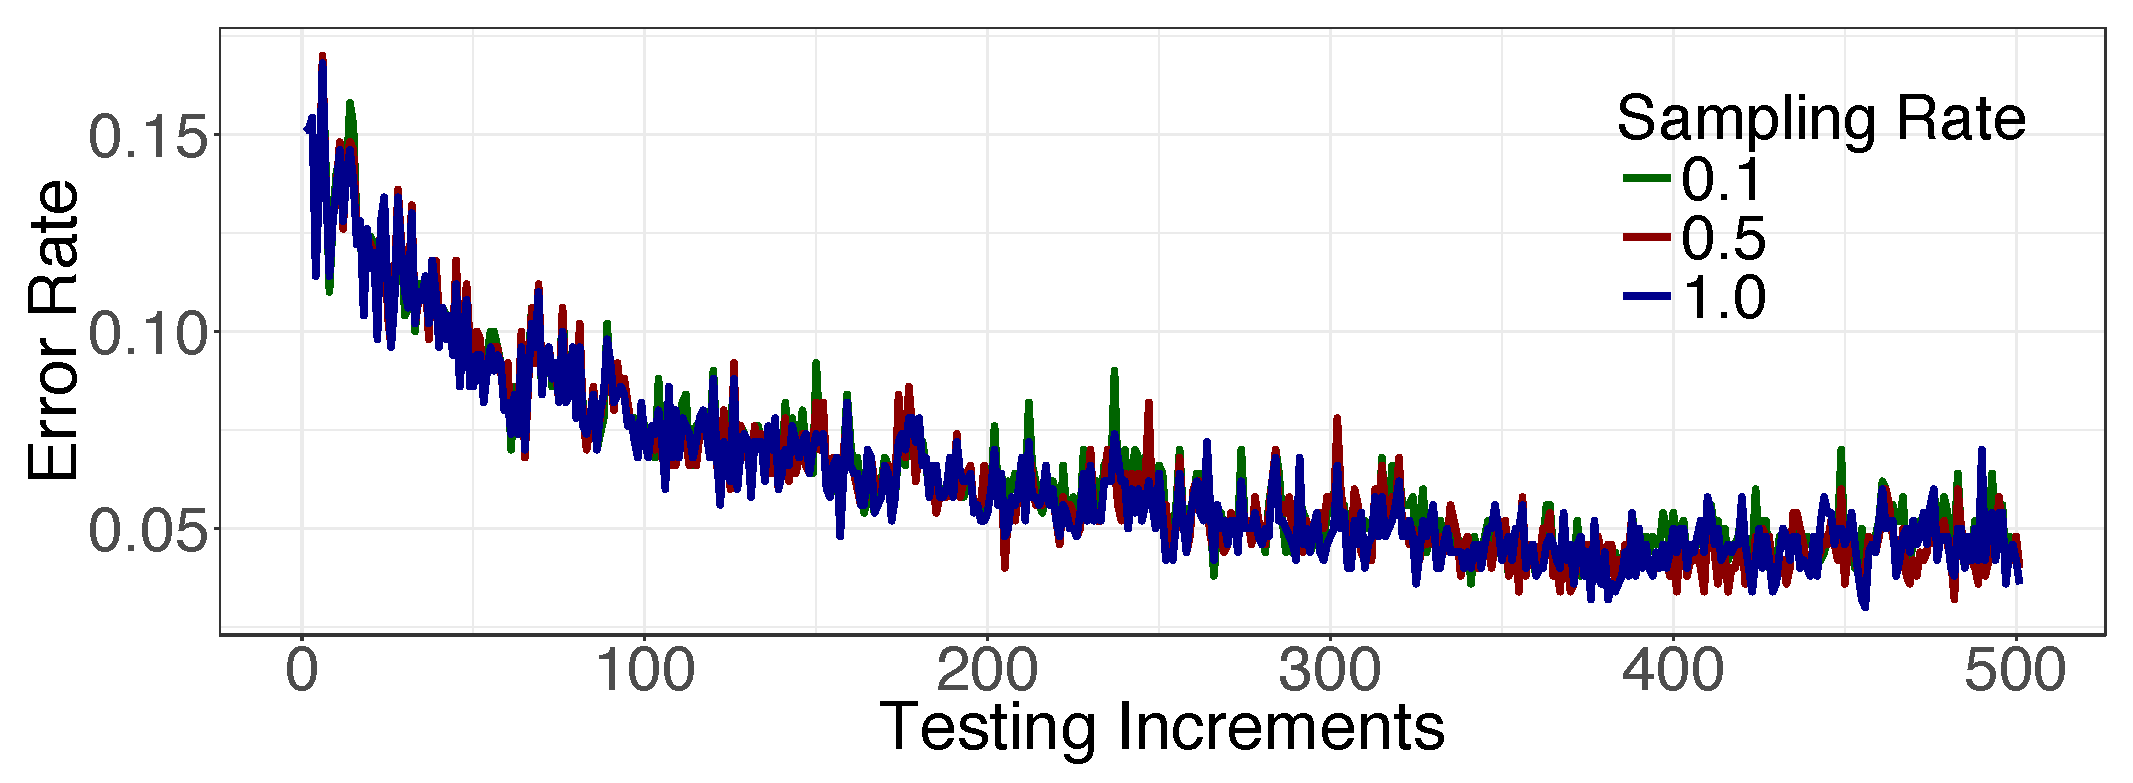
\includegraphics[width=\columnwidth]{../images/experiment-results/mnist-sampling-improved.eps}
\caption{Sampling rate}
\label{fig:mnist-sample-rate}
\end{subfigure}
\begin{subfigure}{\columnwidth}
\centering
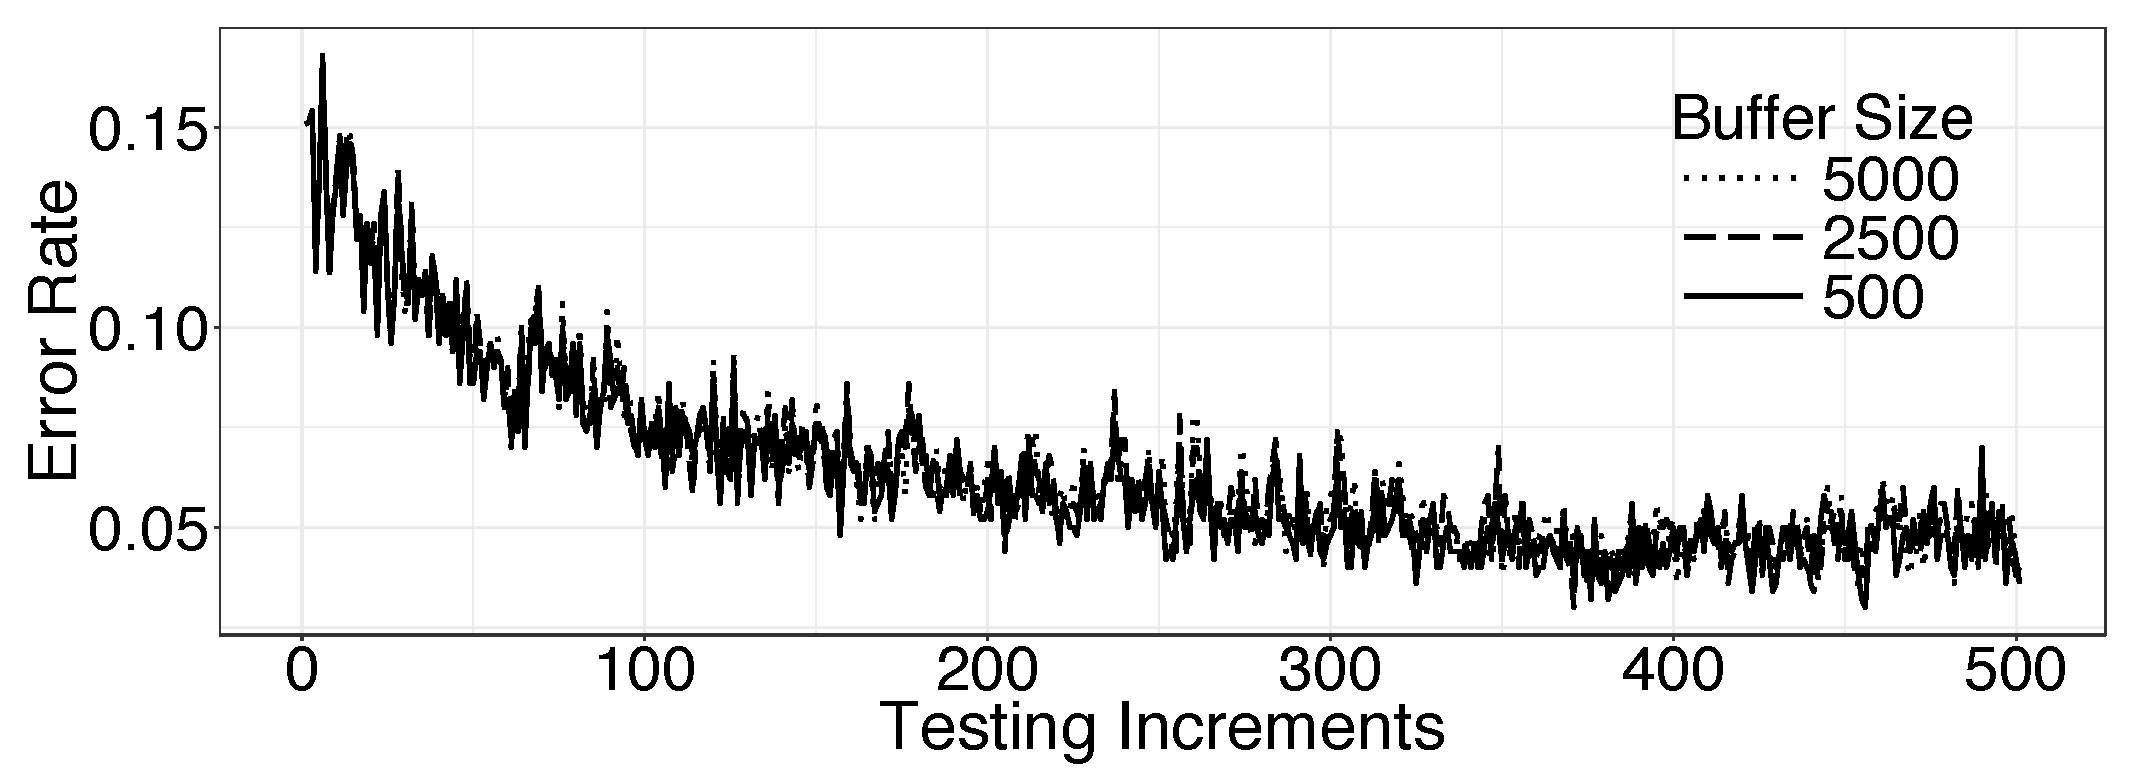
\includegraphics[width=\columnwidth]{../images/experiment-results/mnist-buffersize-improved.eps}
\caption{Buffer size}
\label{fig:mnist-buffer-size}
\end{subfigure}
\vspace{2mm}
\caption{Effect of Sampling and Scheduling Rate on Quality (MNIST)}
\end{figure}

Figure \ref{fig:mnist-buffer-size} shows how the buffer size affects the overall quality of the neural network model.
Similar to the sampling rate case, the error rate of the model is not affected by the scheduling rate.
New training observations that exist in the buffer have the maximum effect on the quality of the model since they are becoming available to the model for the first time.
As the scheduling rate increases, the number of new training observations remain the same, and only the historical data is used more frequently to train the model.
Since neural networks do not gain much benefit by revisiting the same items, increasing the scheduling rate has no effect on the overall quality.

Based on our findings, we conclude that increasing the sampling and scheduling rate does not always affect the quality.
In both the Movie Lens 100k and MNIST datasets, the change in scheduling and sampling rate have small to no effect on the overall quality.
However, the running time of the methods are heavily influenced by these parameters.
\todo[inline]{R3:  Similarly, the treatment of buffer size is also shallow. "Setting these parameters to small values decreases the running time considerably and save computation resources regardless of the type of model the system is serving." What about setting the buffer size as 1? BD: Reviewer's confusion is because I have used both scheduling rate and buffer size in the text, although they both control how often a training iteration is executed, they are 'opposite' of each other. Increasing the scheduling rate means we have a smaller buffer size and decreasing the scheduling rate means we have a bigger buffer size. }
Setting these parameters to small values decreases the running time considerably and save computation resources regardless of the type of model the system is serving.
\subsection{Learning rate adaptation}
A very important parameter of stochastic gradient descent is the learning rate adaptation technique. 
Learning rate controls the degree to which in each iteration SGD the weights are updated.
Momentum \cite{qian1999momentum}, Adam \cite{kingma2014adam}, RMSPROP \cite{tieleman2012lecture}, and AdaDelta \cite{zeiler2012adaptive} are the most effective learning rate tuning methods for stochastic gradient descent. 
However, all of the above methods are defined methods are tested for batch training of the models.
To assess how effective these methods are on hybrid training (scenario C), we experimented the methods on Criteo Dataset.

\begin{figure}[H]
\begin{subfigure}{0.5\columnwidth}
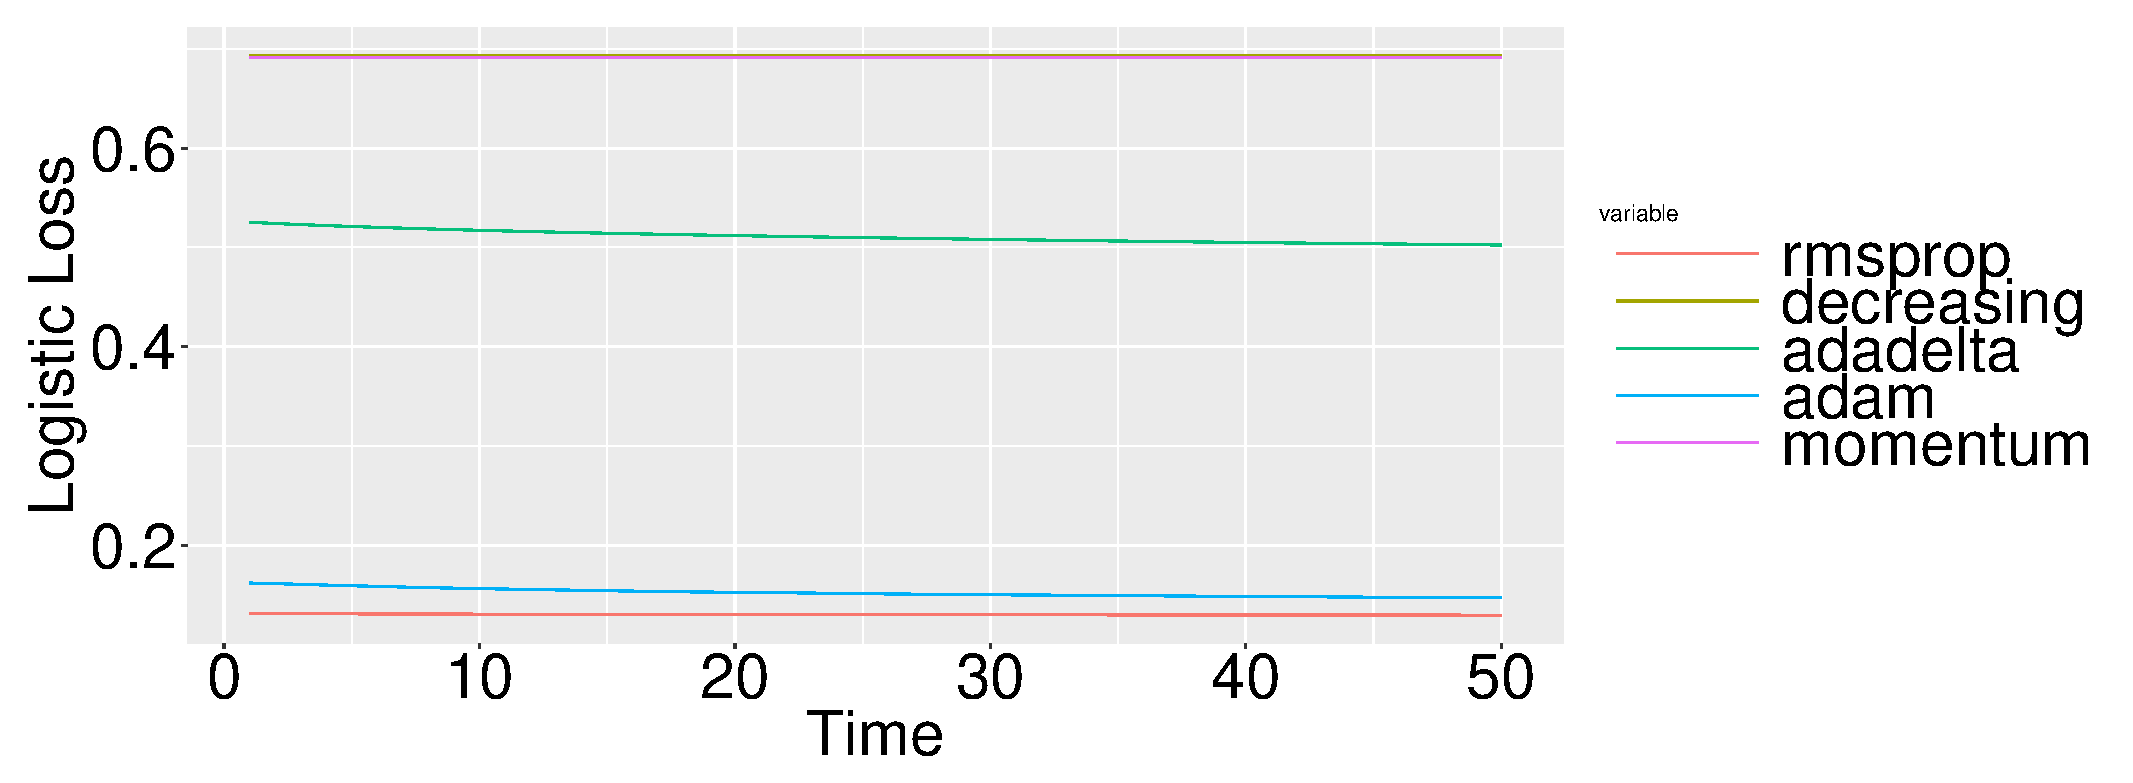
\includegraphics[width=\columnwidth]{../images/experiment-results/criteo-learning-rate-comparison-1.eps}
\caption{}
\label{fig:criteo-learning-rate-1}
\end{subfigure}%
\begin{subfigure}{0.5\columnwidth}
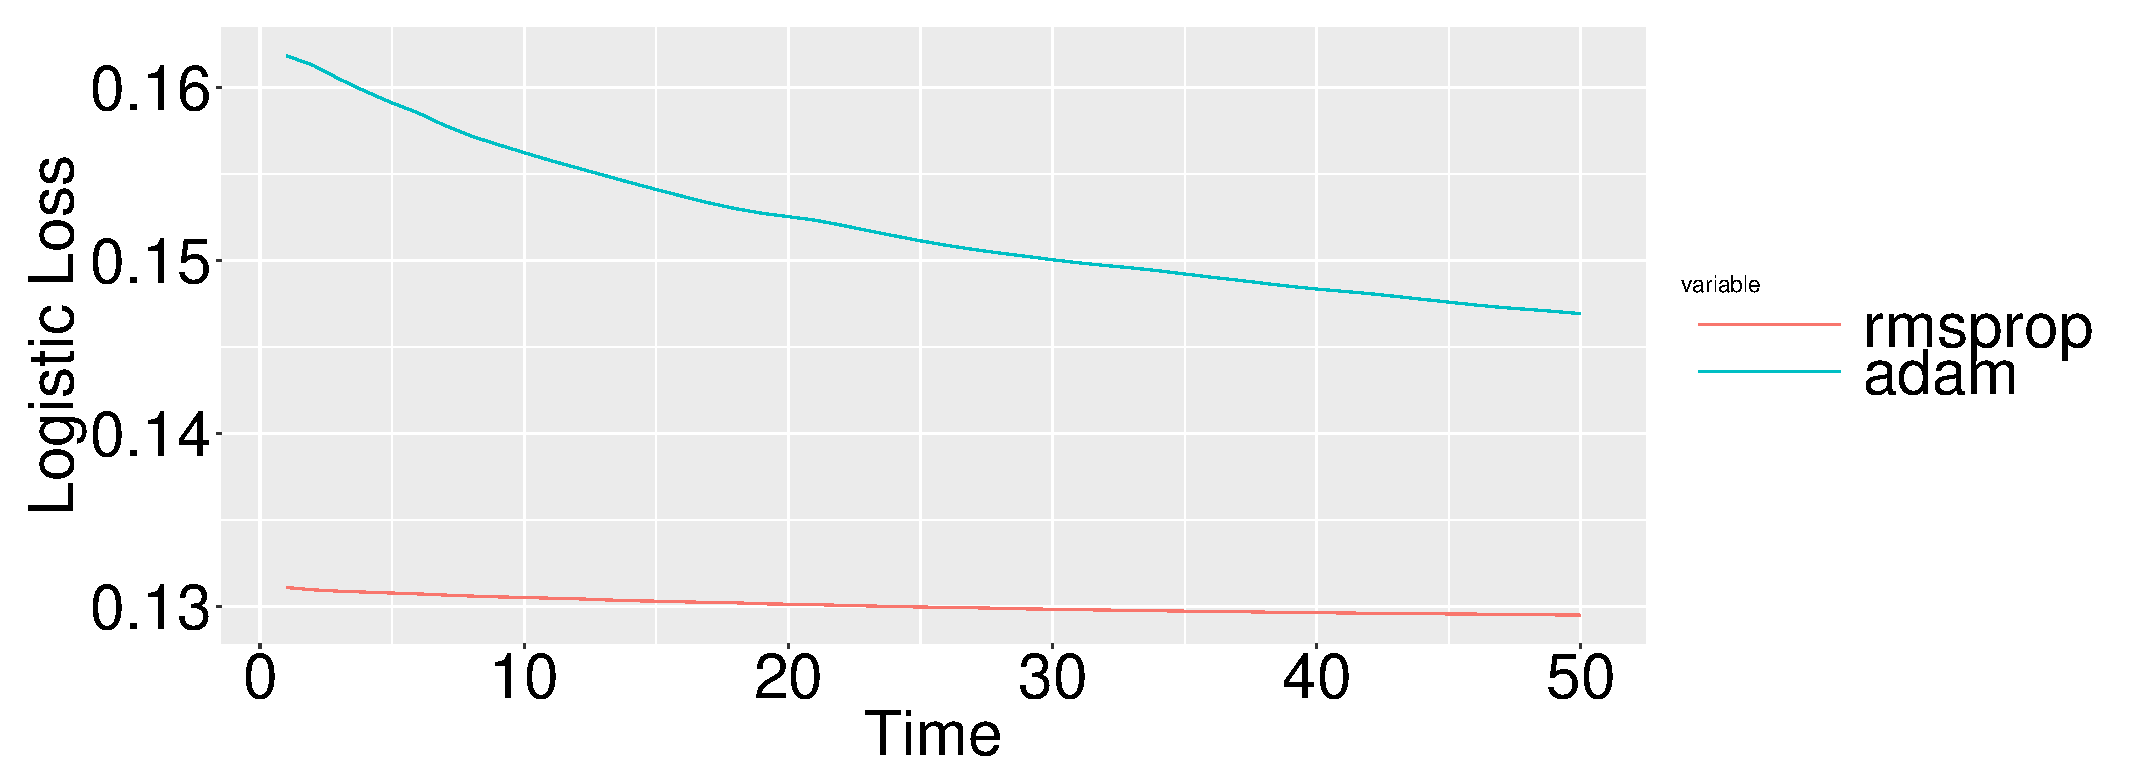
\includegraphics[width=\columnwidth]{../images/experiment-results/criteo-learning-rate-comparison.eps}
\caption{}
\label{fig:criteo-learning-rate}
\end{subfigure}
\vspace{2mm}
\caption{Different Learning rate adaptation methods for Continuous training of Criteo Pipeline}
\end{figure}

Figure \ref{fig:criteo-learning-rate-1} shows the log loss for different learning adaptation methods. 
\todo[inline]{All the methods except for rmsprop and adam seems not work properly without extensive grid search (or not working well at all). I should make sure there's no problem with the code and it is the algorithm that function poorly.}

\subsection{Quality}
Quality achieved continuous compared with retraining method.
\begin{figure}[h]
\centering

\includegraphics[width=\columnwidth]{../images/placeholder.jpeg}
\caption{Log Loss Continuous vs Daily retraining Criteo }
\label{fig:continuous-vs-daily-criteo}
\vspace{2mm}
\end{figure}

\subsection{Training Time}
Total time spent training the pipeline for each scenario.
\begin{figure}[h]
\centering
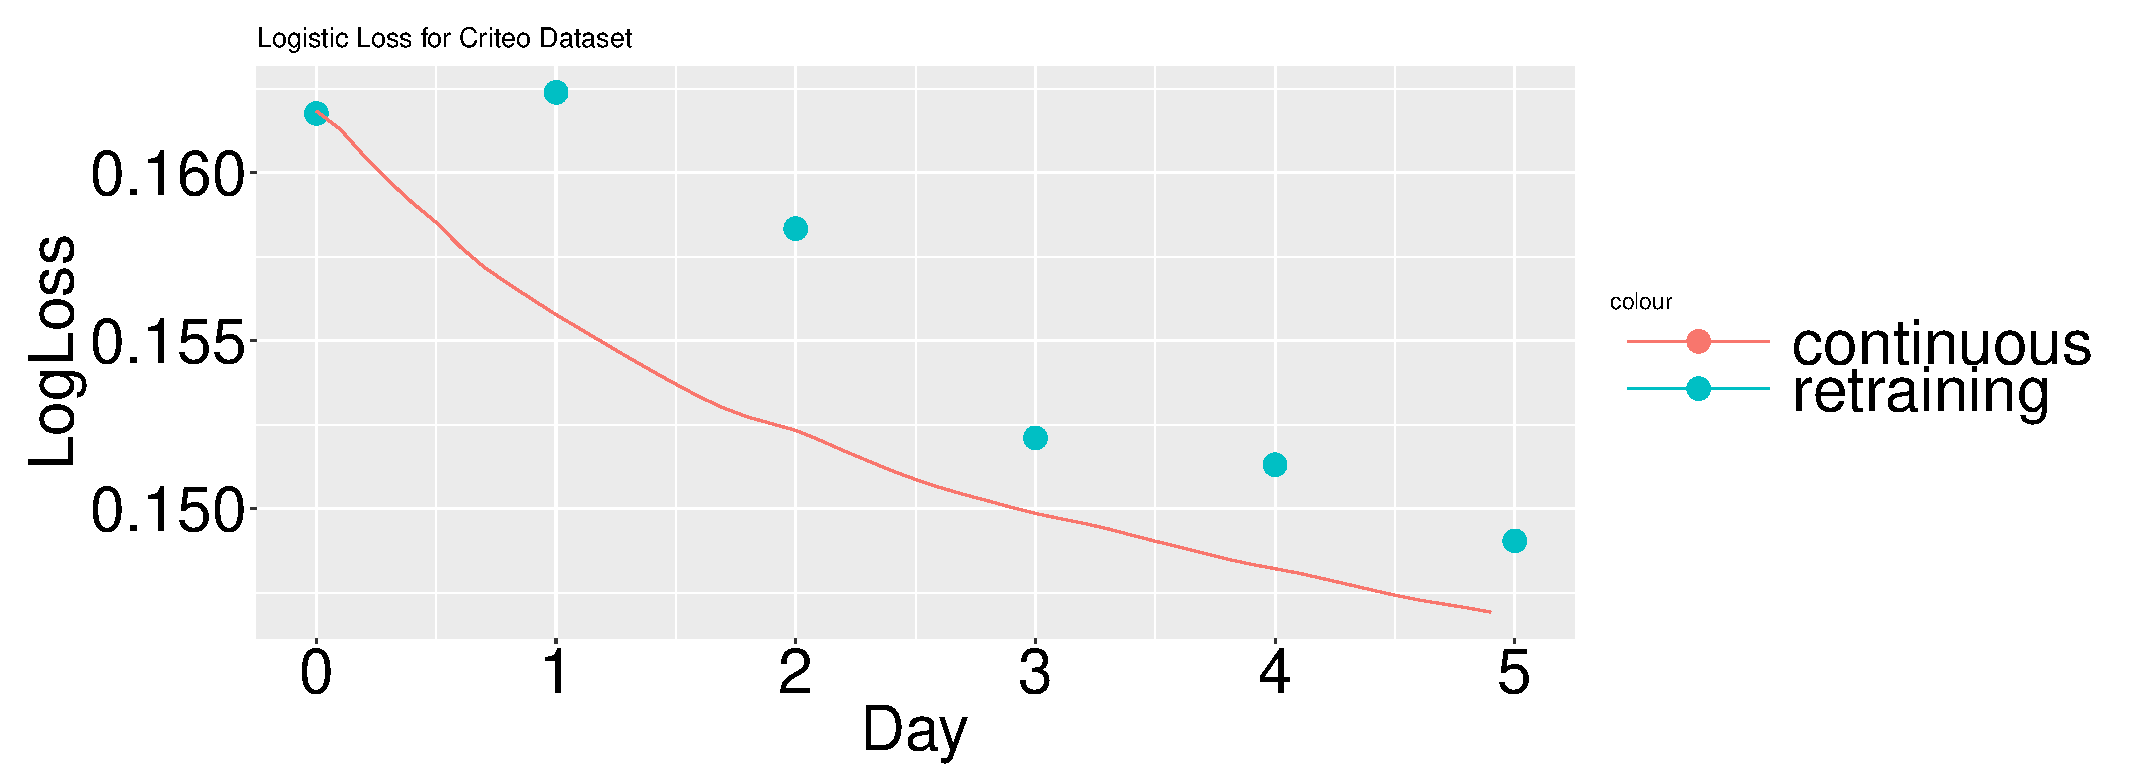
\includegraphics[width=\columnwidth]{../images/experiment-results/criteo-log-loss-continuous-vs-daily.eps}
\caption{Total training time of the pipeline for each scenario}
\label{fig:training-time-criteo}
\vspace{2mm}
\end{figure}
\subsection{Model Freshness}
How recent the pipeline was trained. 
The lower the value, the better quality the predictions are since they are made by a more recent model.
\begin{figure}[h]
\centering

\includegraphics[width=\columnwidth]{../images/placeholder.jpeg}
\caption{Model Freshness for deployment scenarios}
\label{fig:model-freshness-criteo}
\vspace{2mm}
\end{figure}
\subsection{Prediction Latency}


\subsection{Discussion} \label{subsec:discussion}
\begin{figure*}[t]
\begin{subfigure}{0.30\textwidth}
  \centering
  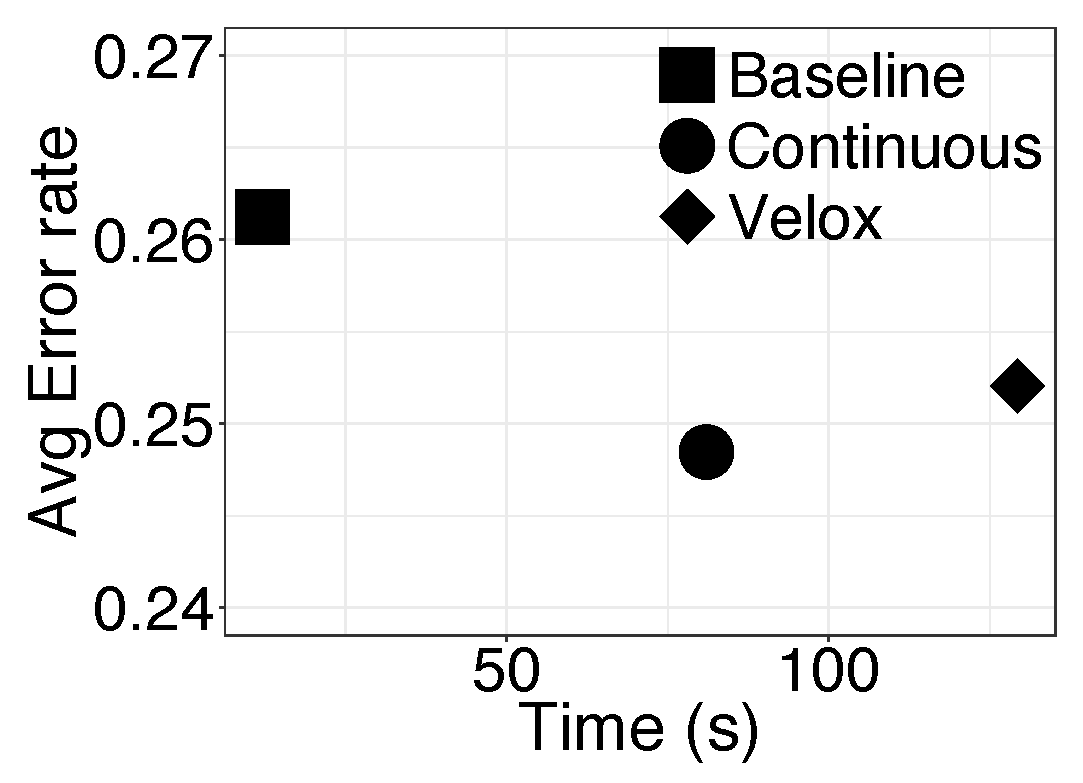
\includegraphics[width=\linewidth]{../images/experiment-results/cover-types-meta-performance.eps}
  \caption{Cover Type}
  \label{subfig:cover-type-meta}
\end{subfigure}%
  \hspace*{10mm}
\begin{subfigure}{0.30\textwidth}
 \centering
  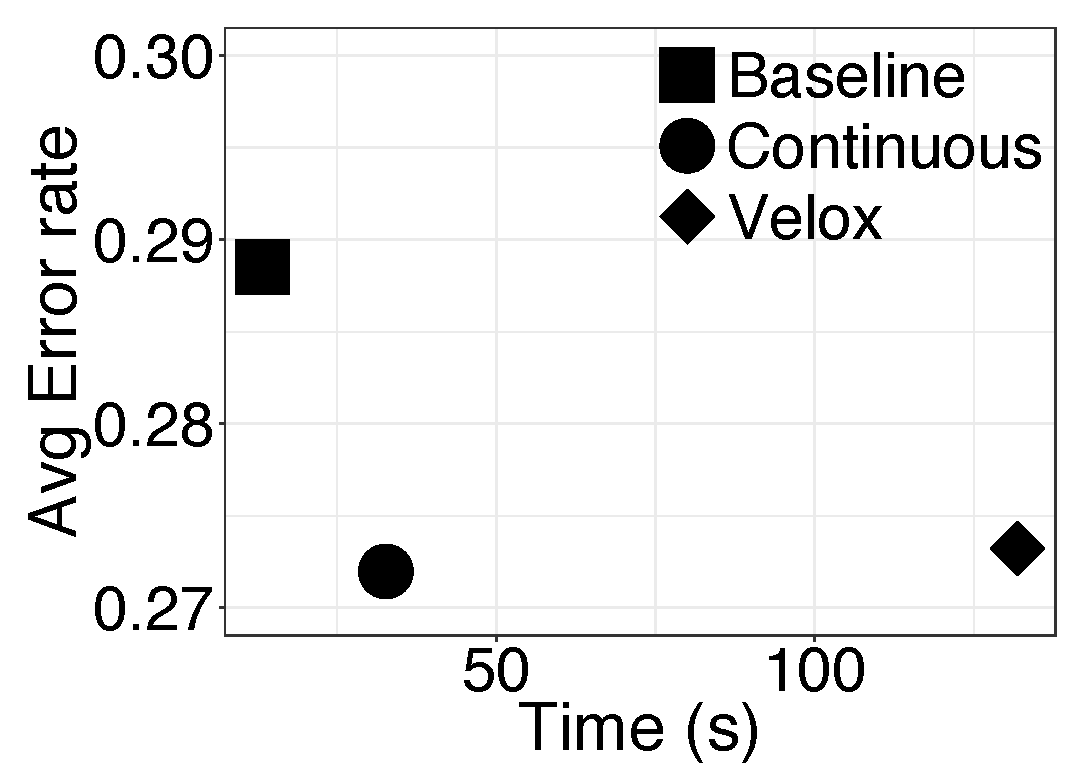
\includegraphics[width=\linewidth]{../images/experiment-results/sea-meta-performance.eps}
  \caption{SEA}
  \label{subfig:sea-meta}
\end{subfigure}%
 \hspace*{10mm}
 \begin{subfigure}{0.30\textwidth}
 \centering
  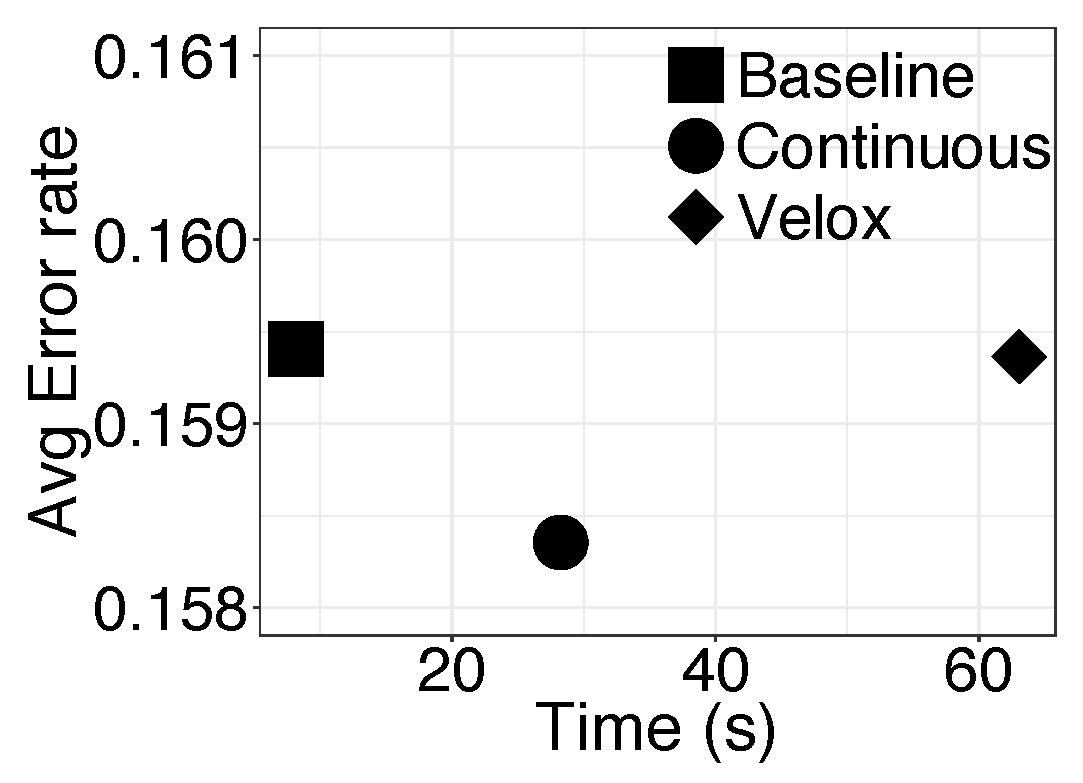
\includegraphics[width=\linewidth]{../images/experiment-results/adult-meta-performance.eps}
  \caption{Adult}
  \label{subfig:adult-meta}
\end{subfigure}%
 \vspace*{5mm}
\centering

\begin{subfigure}{.30\textwidth}
  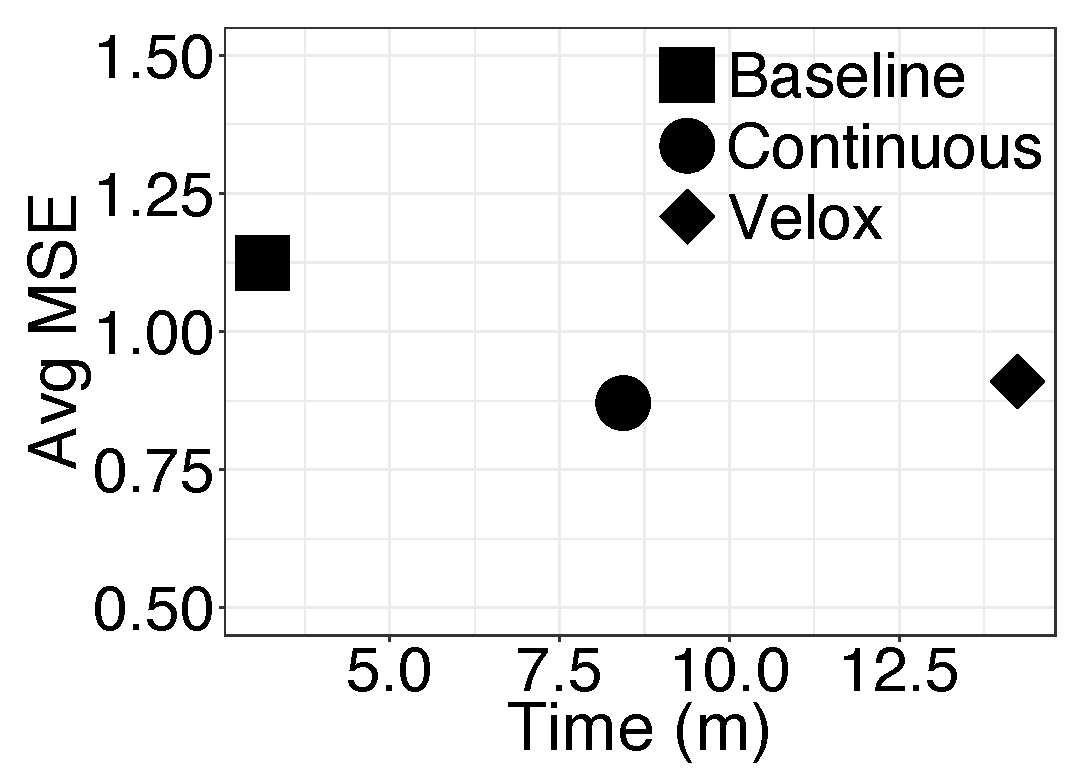
\includegraphics[width=1\linewidth, height=1\linewidth, keepaspectratio]{../images/experiment-results/movie-lens-100k-meta-performance.eps}
  \caption{Movie Lens 100K}
  \label{subfig:movie-lens-100k-meta}
\end{subfigure}%
 \hspace*{10mm}
\begin{subfigure}{0.30\textwidth}
  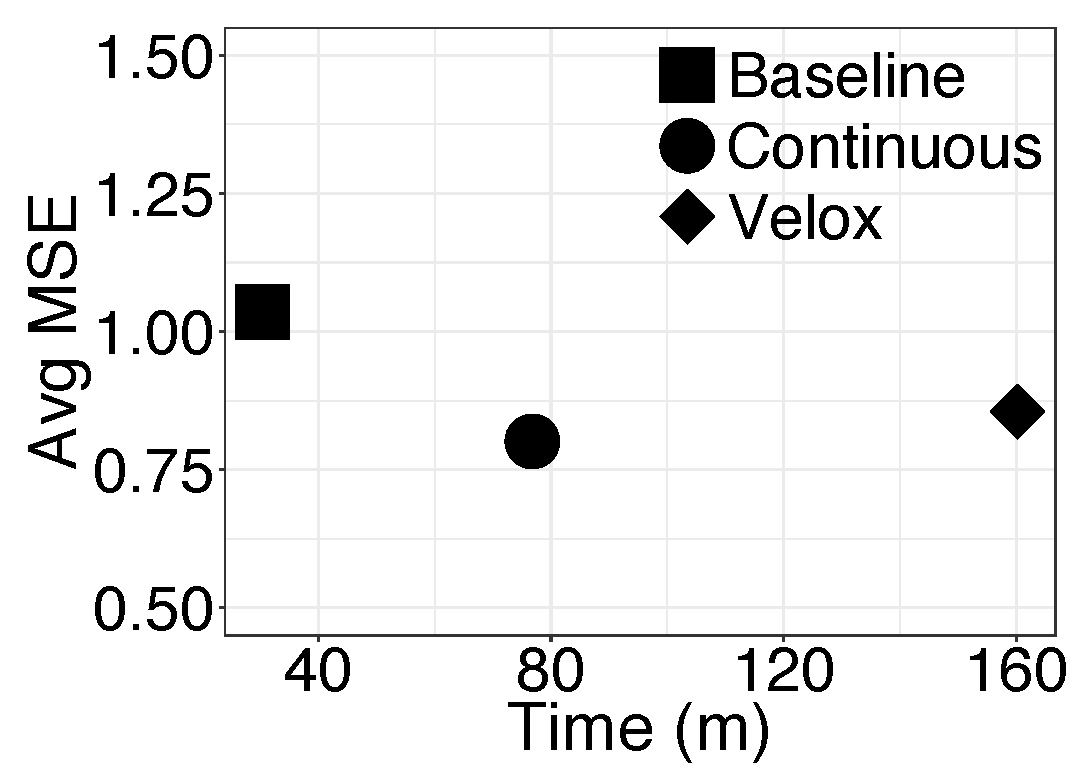
\includegraphics[width=1\linewidth, height=1\linewidth, keepaspectratio]{../images/experiment-results/movie-lens-1m-meta-performance.eps}
  \caption{Movie Lens 1M}
  \label{subfig:movie-lens-1m-meta}
\end{subfigure}


\begin{subfigure}{0.30\textwidth}
  \centering
  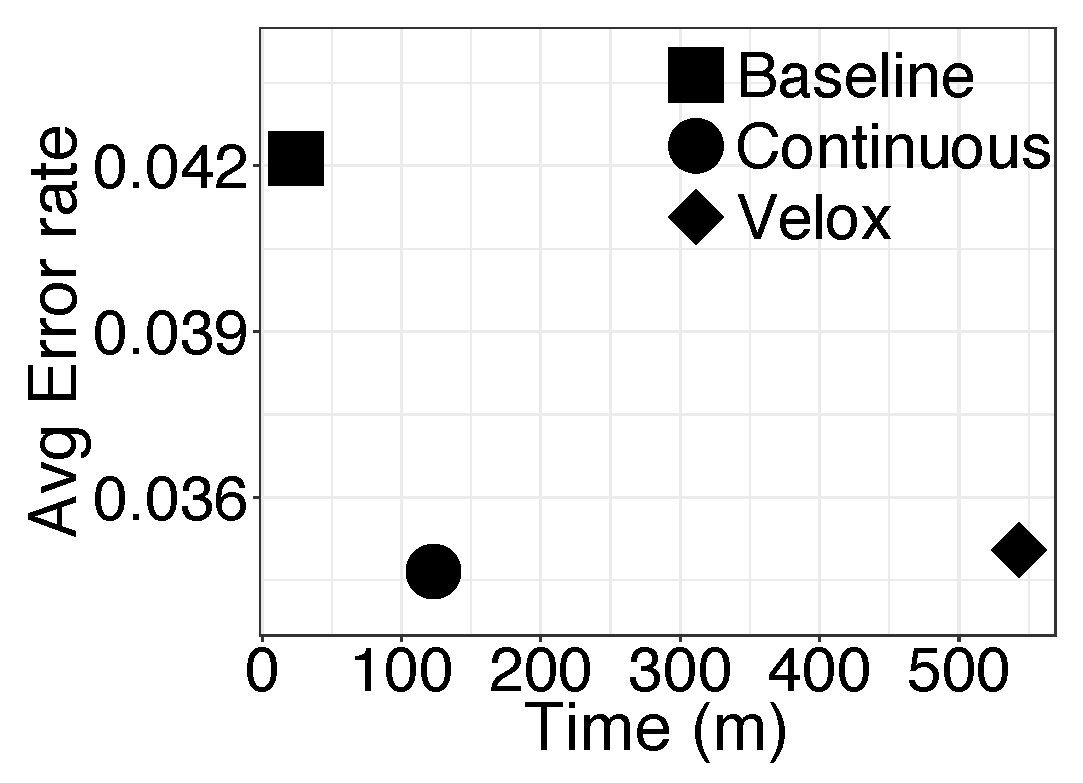
\includegraphics[width=\linewidth]{../images/experiment-results/url-reputation-meta-performance.eps}
  \caption{URL Reputation}
   \label{subfig:url-meta}
\end{subfigure}%
 \hspace*{10mm}
\begin{subfigure}{0.30\textwidth}
 \centering
  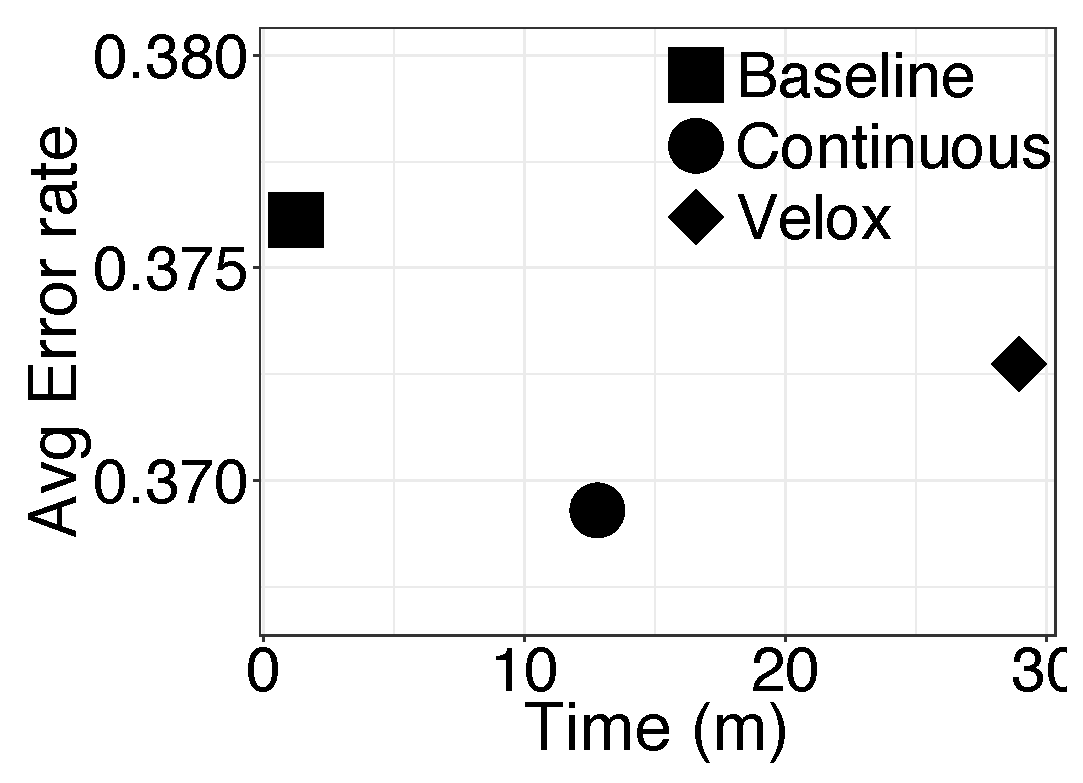
\includegraphics[width=\linewidth]{../images/experiment-results/higgs-meta-performance.eps}
  \caption{Higgs}
   \label{subfig:higgs-meta}
\end{subfigure}
 \vspace*{5mm}
\centering

\vspace{2mm}
\caption{Total Training Time vs Quality}
\label{fig:training-time-vs-quality}
\end{figure*}

Figure \ref{fig:training-time-vs-quality} shows the total training time and average error rate of each of the three different deployment methods (Baseline, Continuous, and Velox) on different datasets.
For all of the evaluated datasets, Continuous achieves the lowest average error rate (for the classification datasets) and average mean squared error (for the recommender system datasets).

The difference in average error rate (or average MSE) between Velox and Continuous is smaller for datasets that contain concept drift (Figure \ref{subfig:sea-meta}, \ref{subfig:movie-lens-100k-meta}, \ref{subfig:movie-lens-1m-meta}, and \ref{subfig:url-meta}).
Since both Velox and Continuous perform incremental and batch training of the model after it is deployed, they both manage to handle the concept drift in the data.
However, Continuous is able to adapt to the changes faster as it is continuously updating the model by executing iterations of SGD.
Since the retraining process is resource intensive, Velox cannot execute it frequently.
As a result, the underlying model in Velox cannot adapt to the changes in the distribution as quickly as Continuous.
The performance of Baseline is very poor in datasets with concept drift.
This is expected, as the underlying model in Baseline is only trained on an initial dataset.
Therefore, it is not capable of adapting to the changes in the data.

Continuous performs very well for datasets with no concept drifts (Figure \ref{subfig:cover-type-meta},  \ref{subfig:adult-meta}, and \ref{subfig:higgs-meta}) as well.
For the Cover Type and Higgs datasets, Baseline does not converge on the initial dataset, therefore it has a higher error rate than Velox and Continuous.
Velox performs better than Baseline on Higgs and Cover Type, however, retraining on these two datasets causes the underlying model to overfit to the existing data.
As a result, the performance of the model is decreased after each retraining.
This leads to an overall lower average error rate than that of Continuous.

As expected, Baseline has the lowest training time for all the datasets since it only trains the model only once on the initial datasets.
The total training time for Continuous is 2 to 5 time smaller than Velox for every datasets.
This has a big impact on prediction latency and accuracy.
In our current prototype, we do not address the problem of the trade off between prediction latency and accuracy.
In our prototype, both prediction and model updates are managed by the same node.
As a result, the prediction component is paused until the SGD iteration (or retraining in the case of Velox) is executed.
Therefore, the system always answers each prediction query using the latest version of the model, although with a much greater delay.
However, in an actual model deployment system, model training and prediction answering are typically executed on separate nodes (or threads).
Therefore, any prediction request arriving at the system is answered immediately, although not with the latest version of the model.
Since the retraining time for Velox is large, a considerable percentage of prediction requests are always answered by an older version of the model.
As a result, while the system is executing a retraining, the error rate will continue to rise until the retraining is finished.
For example in the URL Reputation dataset, the average time of each retraining is 68 minutes in Velox, whereas the average time of each iteration of SGD is 1.5 minutes.
This means that in worst case scenario, the model that is answering a prediction request in Velox is outdated by 1 hour.
Our continuous deployment method reduces this delay since it is updating the underlying model constantly using smaller batches of data.

\section{Conclusions} \label{conclusion}
We propose a system for deploying and maintaining machine learning models that are trained using the SGD optimization method.
Our deployment approach eliminates the need for offline retraining of the model, without affecting the quality.
In our system, we schedule iterations of SGD to run while the machine learning model is answering the prediction queries.
After every iteration, the model is updated with the new parameters.
The frequent updates help in adapting the model to changes in the data distribution.
Moreover, our system is applicable to a wide range of machine learning models as demonstrated in our evaluation.

Our experiments show that the continuous training of the machine learning models is much faster than full retraining, which is the most common approach in deployment and maintenance of machine learning models. 
We show that not only continuous training requires less resources but it also produces models with lower error rates that adapt to the changes in data faster.
Comparing to simple techniques such incremental learning or initial batch training, our technique produces a model with higher quality.

In future work, we will explore more advanced methods for sampling of historical data in order to investigate their effect on the performance of the system. Moreover, we plan to investigate the trade off between prediction latency and prediction accuracy.



\bibliographystyle{plain}

{\fontsize{8}{4}\selectfont \bibliography{main}}
\end{document}